% Options for packages loaded elsewhere
\PassOptionsToPackage{unicode}{hyperref}
\PassOptionsToPackage{hyphens}{url}
%
\documentclass[
]{article}
\usepackage{amsmath,amssymb}
\usepackage{iftex}
\ifPDFTeX
  \usepackage[T1]{fontenc}
  \usepackage[utf8]{inputenc}
  \usepackage{textcomp} % provide euro and other symbols
\else % if luatex or xetex
  \usepackage{unicode-math} % this also loads fontspec
  \defaultfontfeatures{Scale=MatchLowercase}
  \defaultfontfeatures[\rmfamily]{Ligatures=TeX,Scale=1}
\fi
\usepackage{lmodern}
\ifPDFTeX\else
  % xetex/luatex font selection
\fi
% Use upquote if available, for straight quotes in verbatim environments
\IfFileExists{upquote.sty}{\usepackage{upquote}}{}
\IfFileExists{microtype.sty}{% use microtype if available
  \usepackage[]{microtype}
  \UseMicrotypeSet[protrusion]{basicmath} % disable protrusion for tt fonts
}{}
\makeatletter
\@ifundefined{KOMAClassName}{% if non-KOMA class
  \IfFileExists{parskip.sty}{%
    \usepackage{parskip}
  }{% else
    \setlength{\parindent}{0pt}
    \setlength{\parskip}{6pt plus 2pt minus 1pt}}
}{% if KOMA class
  \KOMAoptions{parskip=half}}
\makeatother
\usepackage{xcolor}
\usepackage[margin=1in]{geometry}
\usepackage{color}
\usepackage{fancyvrb}
\newcommand{\VerbBar}{|}
\newcommand{\VERB}{\Verb[commandchars=\\\{\}]}
\DefineVerbatimEnvironment{Highlighting}{Verbatim}{commandchars=\\\{\}}
% Add ',fontsize=\small' for more characters per line
\usepackage{framed}
\definecolor{shadecolor}{RGB}{248,248,248}
\newenvironment{Shaded}{\begin{snugshade}}{\end{snugshade}}
\newcommand{\AlertTok}[1]{\textcolor[rgb]{0.94,0.16,0.16}{#1}}
\newcommand{\AnnotationTok}[1]{\textcolor[rgb]{0.56,0.35,0.01}{\textbf{\textit{#1}}}}
\newcommand{\AttributeTok}[1]{\textcolor[rgb]{0.13,0.29,0.53}{#1}}
\newcommand{\BaseNTok}[1]{\textcolor[rgb]{0.00,0.00,0.81}{#1}}
\newcommand{\BuiltInTok}[1]{#1}
\newcommand{\CharTok}[1]{\textcolor[rgb]{0.31,0.60,0.02}{#1}}
\newcommand{\CommentTok}[1]{\textcolor[rgb]{0.56,0.35,0.01}{\textit{#1}}}
\newcommand{\CommentVarTok}[1]{\textcolor[rgb]{0.56,0.35,0.01}{\textbf{\textit{#1}}}}
\newcommand{\ConstantTok}[1]{\textcolor[rgb]{0.56,0.35,0.01}{#1}}
\newcommand{\ControlFlowTok}[1]{\textcolor[rgb]{0.13,0.29,0.53}{\textbf{#1}}}
\newcommand{\DataTypeTok}[1]{\textcolor[rgb]{0.13,0.29,0.53}{#1}}
\newcommand{\DecValTok}[1]{\textcolor[rgb]{0.00,0.00,0.81}{#1}}
\newcommand{\DocumentationTok}[1]{\textcolor[rgb]{0.56,0.35,0.01}{\textbf{\textit{#1}}}}
\newcommand{\ErrorTok}[1]{\textcolor[rgb]{0.64,0.00,0.00}{\textbf{#1}}}
\newcommand{\ExtensionTok}[1]{#1}
\newcommand{\FloatTok}[1]{\textcolor[rgb]{0.00,0.00,0.81}{#1}}
\newcommand{\FunctionTok}[1]{\textcolor[rgb]{0.13,0.29,0.53}{\textbf{#1}}}
\newcommand{\ImportTok}[1]{#1}
\newcommand{\InformationTok}[1]{\textcolor[rgb]{0.56,0.35,0.01}{\textbf{\textit{#1}}}}
\newcommand{\KeywordTok}[1]{\textcolor[rgb]{0.13,0.29,0.53}{\textbf{#1}}}
\newcommand{\NormalTok}[1]{#1}
\newcommand{\OperatorTok}[1]{\textcolor[rgb]{0.81,0.36,0.00}{\textbf{#1}}}
\newcommand{\OtherTok}[1]{\textcolor[rgb]{0.56,0.35,0.01}{#1}}
\newcommand{\PreprocessorTok}[1]{\textcolor[rgb]{0.56,0.35,0.01}{\textit{#1}}}
\newcommand{\RegionMarkerTok}[1]{#1}
\newcommand{\SpecialCharTok}[1]{\textcolor[rgb]{0.81,0.36,0.00}{\textbf{#1}}}
\newcommand{\SpecialStringTok}[1]{\textcolor[rgb]{0.31,0.60,0.02}{#1}}
\newcommand{\StringTok}[1]{\textcolor[rgb]{0.31,0.60,0.02}{#1}}
\newcommand{\VariableTok}[1]{\textcolor[rgb]{0.00,0.00,0.00}{#1}}
\newcommand{\VerbatimStringTok}[1]{\textcolor[rgb]{0.31,0.60,0.02}{#1}}
\newcommand{\WarningTok}[1]{\textcolor[rgb]{0.56,0.35,0.01}{\textbf{\textit{#1}}}}
\usepackage{graphicx}
\makeatletter
\def\maxwidth{\ifdim\Gin@nat@width>\linewidth\linewidth\else\Gin@nat@width\fi}
\def\maxheight{\ifdim\Gin@nat@height>\textheight\textheight\else\Gin@nat@height\fi}
\makeatother
% Scale images if necessary, so that they will not overflow the page
% margins by default, and it is still possible to overwrite the defaults
% using explicit options in \includegraphics[width, height, ...]{}
\setkeys{Gin}{width=\maxwidth,height=\maxheight,keepaspectratio}
% Set default figure placement to htbp
\makeatletter
\def\fps@figure{htbp}
\makeatother
\setlength{\emergencystretch}{3em} % prevent overfull lines
\providecommand{\tightlist}{%
  \setlength{\itemsep}{0pt}\setlength{\parskip}{0pt}}
\setcounter{secnumdepth}{-\maxdimen} % remove section numbering
\ifLuaTeX
  \usepackage{selnolig}  % disable illegal ligatures
\fi
\usepackage{bookmark}
\IfFileExists{xurl.sty}{\usepackage{xurl}}{} % add URL line breaks if available
\urlstyle{same}
\hypersetup{
  pdftitle={AR-MA manual},
  hidelinks,
  pdfcreator={LaTeX via pandoc}}

\title{AR-MA manual}
\author{}
\date{\vspace{-2.5em}2023-09-16}

\begin{document}
\maketitle

\subsection{White Noise}\label{white-noise}

Pembangkitan data berpola AR, MA, ARMA, dan banyak proses deret waktu
lainnya diawali pembangkitan \emph{white noise}. \emph{White noise}
merupakan sederet nilai dari peubah bebas stokastik identik. Oleh karena
itu, \emph{white noise} memiliki dua karakteristik penting:

\begin{enumerate}
\def\labelenumi{\arabic{enumi}.}
\tightlist
\item
  \emph{White noise} tidak memiliki autokorelasi (\textbf{karena saling
  bebas})
\item
  Nilai harapan dan ragam \emph{white noise} sama (\textbf{karena
  berasal dari peubah acak bebas stokastik identik})
\end{enumerate}

\emph{White noise} dibangkitkan dari suatu peubah acak, umumnya peubah
acak normal.

\begin{Shaded}
\begin{Highlighting}[]
\NormalTok{wn }\OtherTok{\textless{}{-}} \FunctionTok{rnorm}\NormalTok{(}\DecValTok{200}\NormalTok{)}
\FunctionTok{ts.plot}\NormalTok{(wn)}
\end{Highlighting}
\end{Shaded}

\includegraphics{Pertemuan-4---Pembangkitan-Arma_files/figure-latex/unnamed-chunk-1-1.pdf}

Dapat terlihat bahwa \emph{white noise} tidak memiliki autokorelasi dari
ACF. Perhatikan bahwa lag ke-0 adalah korelasi observasi ke-t dengan
dirinya sendiri. Nilai korelasi tersebut pasti 1. Sebagai alternatif,
lag pertama di plot ACF dapat ditetapkan sebagai 1 (alih-alih 0) dengan
menambahkan argumen \texttt{xlim(1,\ lag\ akhir)}. Plot tersebut dapat
disandingkan bersamaan dengan membuat matriks \(1 \times 2\) dengan
\texttt{par(mfrow\ =\ c(1,2))}.

\begin{Shaded}
\begin{Highlighting}[]
\FunctionTok{par}\NormalTok{(}\AttributeTok{mfrow =} \FunctionTok{c}\NormalTok{(}\DecValTok{1}\NormalTok{, }\DecValTok{2}\NormalTok{)) }
\FunctionTok{acf}\NormalTok{(wn)}
\FunctionTok{acf}\NormalTok{(wn, }\AttributeTok{xlim =} \FunctionTok{c}\NormalTok{(}\DecValTok{1}\NormalTok{, }\DecValTok{20}\NormalTok{))}
\end{Highlighting}
\end{Shaded}

\includegraphics{Pertemuan-4---Pembangkitan-Arma_files/figure-latex/unnamed-chunk-2-1.pdf}

\subsection{Proses MA}\label{proses-ma}

Proses MA dapat dituliskan sebagai berikut:

\[
y_{t} = c + e_t + \theta_{1}e_{t-1} + \theta_{2}e_{t-2} + \dots + \theta_{q}e_{t-q} = c+{e_t+\sum_{i=1}^p \theta_ie_{t-i}}
\] Terlihat bahwa \(e_t\), atau \emph{white noise}, berperan penting
dalam pembangkitan proses MA.

\subsection{Pembangkitan Proses MA(1)}\label{pembangkitan-proses-ma1}

Akan dicoba membangkitkan proses MA paling sederhana, yaitu MA(1) dengan
\(\theta = 0.5\) sebanyak 200 observasi dan \(c=0\). Karena diperlukan
satu nilai awal untuk \(e_{t-1}\), masukkan nilai pertama white noise
sebagai nilai awal tersebut.

\begin{Shaded}
\begin{Highlighting}[]
\FunctionTok{set.seed}\NormalTok{(}\DecValTok{1234}\NormalTok{)}
\NormalTok{ma }\OtherTok{\textless{}{-}}\NormalTok{ wn[}\DecValTok{1}\NormalTok{]}
\end{Highlighting}
\end{Shaded}

Nilai-nilai selanjutnya dapat dicari melalui \emph{loop}. Bentuk loop
dapat dilihat dari rumus MA(1) yang hendak dibangkitkan:

\[
y_t = e_t+0.5e_{t-1}
\]

\begin{Shaded}
\begin{Highlighting}[]
\ControlFlowTok{for}\NormalTok{(i }\ControlFlowTok{in} \DecValTok{2}\SpecialCharTok{:}\DecValTok{200}\NormalTok{)\{}
\NormalTok{   ma[i] }\OtherTok{\textless{}{-}}\NormalTok{ wn[i] }\SpecialCharTok{+} \FloatTok{0.5} \SpecialCharTok{*}\NormalTok{ wn[i }\SpecialCharTok{{-}} \DecValTok{1}\NormalTok{] }
\NormalTok{\}}
\NormalTok{ma}
\end{Highlighting}
\end{Shaded}

\begin{verbatim}
##   [1] -0.282228699 -0.243217090 -0.397884461 -0.585427549 -0.451548804
##   [6] -0.347290574  2.068107579  1.673124569  1.007617549 -0.079613254
##  [11] -0.912202596 -1.877671705  0.650956207 -0.474140987  0.138135971
##  [16]  0.385199305  1.424495294  1.840720933  0.829766992  0.503688630
##  [21]  1.084366537  1.286684380 -1.056788854 -0.780557233  0.305263927
##  [26]  0.555770225  0.712164846  0.016944590  0.122664292 -0.967065582
##  [31] -0.131721054  0.982799932  1.587888689  2.129164197  1.817571498
##  [36] -1.063639381 -0.386214693 -0.460489222 -0.746579550  0.365462192
##  [41]  0.377859425 -0.213150041 -0.405990047  1.505302353  0.501948910
##  [46] -0.116918662 -1.492788833  0.509737651  0.917952817 -0.097513113
##  [51] -0.288104535 -0.525459756  1.393915835  0.551460755 -0.034596293
##  [56] -1.626642920 -1.544086462 -1.368683909 -0.380078710  0.611664578
##  [61] -1.660243129 -0.886992172 -0.254342241  0.899784660  0.766188862
##  [66] -1.761972049 -0.070742120  0.305284605 -0.143680249 -0.287373981
##  [71] -0.134257094 -0.379718097 -0.601010400 -0.153355362 -0.246344412
##  [76] -0.968957183 -1.249331370 -1.024985534 -1.016929709 -0.013372591
##  [81] -0.927204611  0.048951806  1.340941722  1.169039669  2.800505037
##  [86]  1.091764473  1.842362051  0.618020942 -0.296680446  1.105712948
##  [91] -1.730679920 -0.534535248  0.407543706  1.427463168  1.224874710
##  [96]  0.865818748  1.124230474  0.471705581 -0.007347636 -1.304706629
## [101] -1.568286771 -1.011229002 -1.176883184  1.846269701  2.083265413
## [106]  1.828070518 -2.124535589 -1.246987011 -0.812642784  0.274127224
## [111]  0.030145849  0.192097260  1.380748227  0.853748404 -0.450106532
## [116]  0.880603074  1.173566939  0.110078537 -0.211501318 -2.083794481
## [121] -2.006541477 -0.217088380  0.854317264 -1.063338793  0.870564527
## [126] -0.471889416 -2.787492309 -2.281086823  0.068180687 -0.070349074
## [131]  0.607802121  1.193082330  0.060878681 -0.623656506  0.971841198
## [136] -0.347573654  1.555079021 -0.444157497 -1.521519822  1.097116005
## [141]  2.561307727  0.958748261  1.566734018  0.803963443  0.385629423
## [146] -1.606852221 -1.970352857 -0.117032687  0.152503837 -1.055126810
## [151] -1.308650440 -2.526212483 -1.583152898 -1.729129864 -0.198243810
## [156] -0.242465624 -1.684225889 -1.361084575 -1.015131936 -0.386164356
## [161] -0.771800576 -0.535923261  0.266683383  1.905328614 -0.095715380
## [166] -1.727309694 -1.722229065 -0.792850493 -0.106868884 -1.364471713
## [171] -0.041902965  0.670188779  3.045629846  2.296497964 -0.375540491
## [176]  1.140207338  0.257146140 -0.572136032  0.745855297 -2.147981107
## [181] -1.044812639  0.995196777  2.701121025  1.804704113  1.279766757
## [186] -1.130794955 -1.373435850 -1.756710274  0.480154224  0.336990298
## [191] -0.596509447  0.670167684  0.513667659  1.028053217  2.513771572
## [196]  1.034448047  0.751039569  0.355254765 -0.715495952 -1.318049571
\end{verbatim}

Selain menggunakan cara di atas, pembangkitan proses MA(1) dapat
dilakukan dengan fungsi \texttt{arima.sim()} sebagai berikut.

\begin{Shaded}
\begin{Highlighting}[]
\NormalTok{ma1 }\OtherTok{\textless{}{-}} \FunctionTok{arima.sim}\NormalTok{(}\FunctionTok{list}\NormalTok{(}\AttributeTok{order=}\FunctionTok{c}\NormalTok{(}\DecValTok{0}\NormalTok{,}\DecValTok{0}\NormalTok{,}\DecValTok{1}\NormalTok{), }\AttributeTok{ma=}\FloatTok{0.5}\NormalTok{), }\AttributeTok{n=}\DecValTok{200}\NormalTok{)}
\NormalTok{ma1}
\end{Highlighting}
\end{Shaded}

\begin{verbatim}
## Time Series:
## Start = 1 
## End = 200 
## Frequency = 1 
##   [1] -0.326103633  1.223155798 -1.803477114 -0.743724163  0.720618237
##   [6] -0.321712014 -0.834001836 -0.837767927 -1.172263829 -0.922211614
##  [11] -1.236982795 -1.275447117 -0.323668130  0.991723468  0.369461535
##  [16] -0.566152253 -1.166700170 -1.292769389  1.997249338  1.342005809
##  [21] -0.423641787 -0.685890821  0.239315505 -0.463925526 -1.795065034
##  [26] -0.149346734 -0.736277863 -0.526966162 -0.943517751  0.634323246
##  [31]  0.075555694 -0.947236577 -0.855978079 -1.879722499 -1.982165997
##  [36] -2.763849280 -2.431013017 -0.964790455 -0.613044470  1.216547495
##  [41] -0.343894591 -1.389685996 -0.708305319 -1.134651577 -1.465684356
##  [46] -1.591575352 -1.805644982 -1.149821062 -0.758764017 -2.054456235
##  [51] -1.485091553 -1.399927587 -1.569406822 -0.669790528  0.481901057
##  [56]  1.929345382  0.050555312  1.219232917 -0.354853733  0.077684190
##  [61]  2.877285303  1.239735146 -0.687013775 -0.342421546  1.773282070
##  [66] -0.250065513  0.798523311  2.013478380  1.001255193  0.175129237
##  [71] -0.452022319 -0.594258302  0.465024601  2.394414145  0.881737018
##  [76] -1.467400153 -1.418932250 -0.103529126 -0.187928234 -0.336319515
##  [81] -0.258889056 -1.457298924 -0.859938113  0.763338672  1.122724840
##  [86]  0.898801707 -0.127733300 -0.392959758 -1.290324765 -0.650422759
##  [91]  0.228616592  1.833562008  1.854495256  0.005173183  0.107758575
##  [96] -0.956832895  0.310899605  1.412018567  2.607575482  1.475082087
## [101] -0.267456706 -0.171365743 -0.469481036 -1.077237478 -0.246010014
## [106] -0.812769986 -0.279946925  0.439060955  0.125379014 -0.221987177
## [111] -0.747037061 -1.434302107  0.294390587  0.446999627  0.842321880
## [116] -0.828717543 -0.453117512  0.757679514  0.310306777 -0.204530357
## [121] -0.877602731  1.667208664  1.779582447  2.199459029  0.992163792
## [126] -0.591379478 -1.828992770 -1.392743891 -0.091748383  1.126841114
## [131]  0.759595309 -1.045573245  0.082740172 -1.315743771 -1.190902716
## [136] -0.499044453 -2.106305212 -0.054065501 -0.162842834 -0.645472447
## [141]  1.228129568  1.334248357  0.209905509  0.459546930  0.656153196
## [146]  1.862492351  1.107321627  0.644219325  0.600688287 -0.203461660
## [151] -0.090999361  1.687554377 -0.056220152 -0.316036238  1.423010660
## [156]  0.446444243 -1.170693351 -1.396475010 -0.825018832 -1.042413588
## [161] -0.684314429 -0.544739402 -0.390260651  0.315530699  0.828161177
## [166]  1.990522308  0.770409218 -0.355186739  1.310585761  2.439832256
## [171]  0.895408736 -0.311035300 -1.988564077  0.500144690 -0.131951235
## [176] -1.542554011  2.481884489  1.756904251  0.084252044 -2.748848828
## [181] -1.465900350  0.926136441  0.901884783  1.119256619  2.439893281
## [186]  2.160974614  0.075817242  0.449811671  0.153673815 -0.637278926
## [191] -3.124794049 -2.217526180  0.092991209  2.411939857  1.584710884
## [196]  0.870557511 -0.655798108 -0.320296897 -1.996910188 -0.553891950
\end{verbatim}

\subsection{Karakteristik MA(1)}\label{karakteristik-ma1}

\subsubsection{Plot Time Series}\label{plot-time-series}

\begin{Shaded}
\begin{Highlighting}[]
\FunctionTok{ts.plot}\NormalTok{(ma)}
\end{Highlighting}
\end{Shaded}

\includegraphics{Pertemuan-4---Pembangkitan-Arma_files/figure-latex/unnamed-chunk-6-1.pdf}

Berdasarkan plot time series, terlihat bahwa data MA(1) yang
dibangkitkan stasioner dalam rataan

\subsubsection{Plot ACF}\label{plot-acf}

\begin{Shaded}
\begin{Highlighting}[]
\FunctionTok{acf}\NormalTok{(ma,}\AttributeTok{lag.max =} \DecValTok{20}\NormalTok{)}
\end{Highlighting}
\end{Shaded}

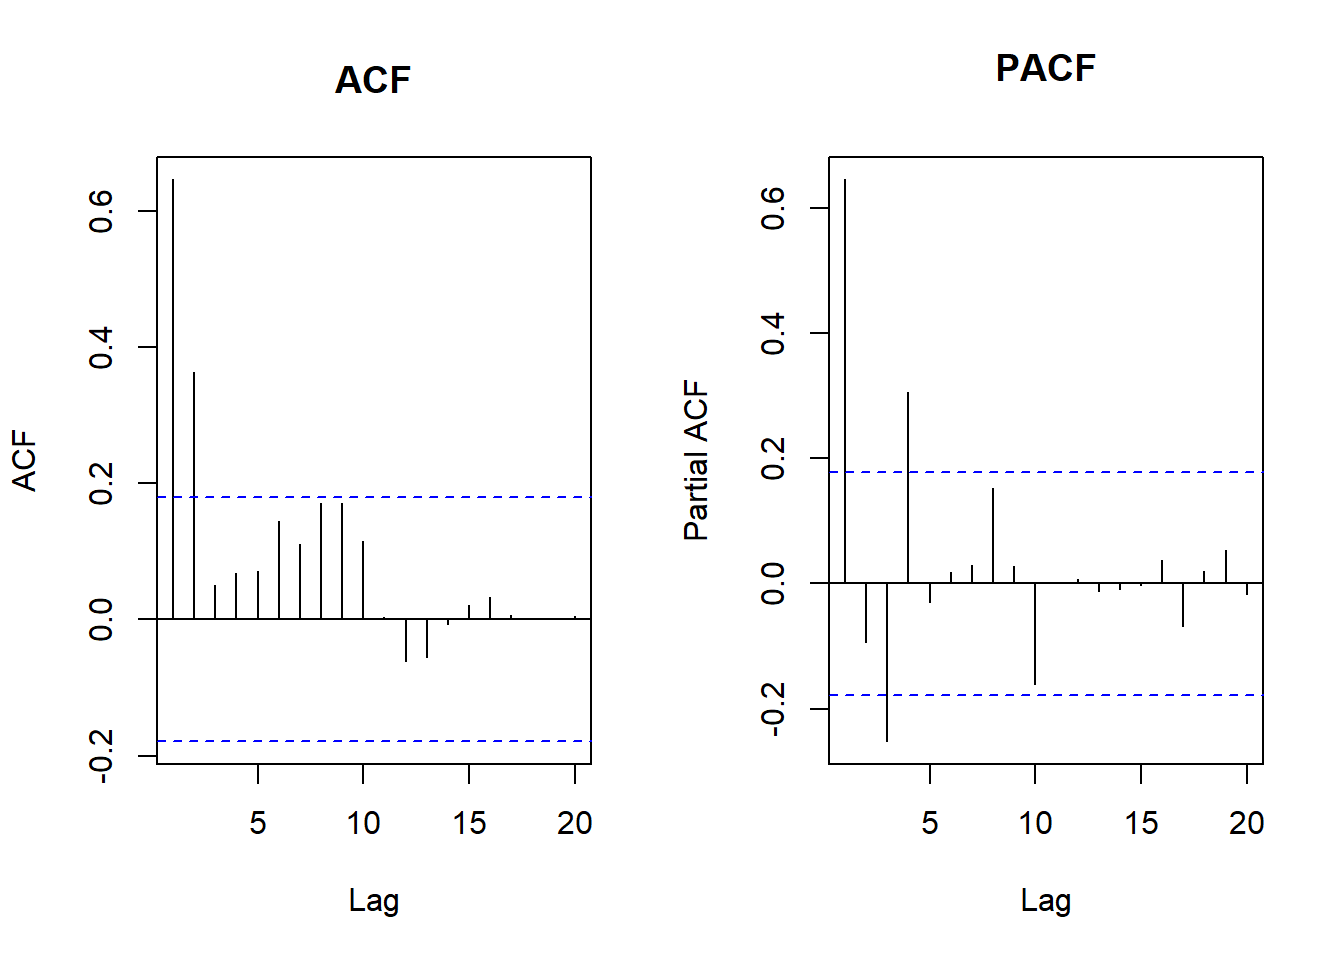
\includegraphics{Pertemuan-4---Pembangkitan-Arma_files/figure-latex/unnamed-chunk-7-1.pdf}

Berdasarkan plot AFC tersebut, terlihat bahwa plot ACF \emph{cuts off}
di lag pertama

\subsubsection{Plot PACF}\label{plot-pacf}

\begin{Shaded}
\begin{Highlighting}[]
\FunctionTok{pacf}\NormalTok{(ma)}
\end{Highlighting}
\end{Shaded}

\includegraphics{Pertemuan-4---Pembangkitan-Arma_files/figure-latex/unnamed-chunk-8-1.pdf}

Berdasarkan plot PACF tersebut, terlihat bahwa plot PACF cenderung
\emph{tails off} dan membentuk gelombang sinus

\subsubsection{Plot EACF}\label{plot-eacf}

\begin{Shaded}
\begin{Highlighting}[]
\NormalTok{TSA}\SpecialCharTok{::}\FunctionTok{eacf}\NormalTok{(ma)}
\end{Highlighting}
\end{Shaded}

\begin{verbatim}
## AR/MA
##   0 1 2 3 4 5 6 7 8 9 10 11 12 13
## 0 x o o o o o o o o o o  o  o  o 
## 1 x x o o o o o o o o o  o  o  o 
## 2 x o o o o o o o o o o  o  o  o 
## 3 x o o o o o o o o o o  o  o  o 
## 4 x x o o o o o o o o o  o  o  o 
## 5 x x x o o o o o o o o  o  o  o 
## 6 o x x o x o o o o o o  o  o  o 
## 7 o x o o x o o o o o o  o  o  o
\end{verbatim}

Berdasarkan pola segitiga nol pada plot EACF, terlihat bahwa segitiga
nol berada pada ordo AR(0) dan ordo MA(1)

\subsubsection{Scatterplot Antar Lag}\label{scatterplot-antar-lag}

\paragraph{\texorpdfstring{Korelasi antara \(Y_t\) dengan
\(Y_{t-1}\)}{Korelasi antara Y\_t dengan Y\_\{t-1\}}}\label{korelasi-antara-y_t-dengan-y_t-1}

\begin{Shaded}
\begin{Highlighting}[]
\CommentTok{\#Yt}
\NormalTok{yt\_ma }\OtherTok{\textless{}{-}}\NormalTok{ ma[}\SpecialCharTok{{-}}\DecValTok{1}\NormalTok{]}
\NormalTok{yt\_ma}
\end{Highlighting}
\end{Shaded}

\begin{verbatim}
##   [1] -0.243217090 -0.397884461 -0.585427549 -0.451548804 -0.347290574
##   [6]  2.068107579  1.673124569  1.007617549 -0.079613254 -0.912202596
##  [11] -1.877671705  0.650956207 -0.474140987  0.138135971  0.385199305
##  [16]  1.424495294  1.840720933  0.829766992  0.503688630  1.084366537
##  [21]  1.286684380 -1.056788854 -0.780557233  0.305263927  0.555770225
##  [26]  0.712164846  0.016944590  0.122664292 -0.967065582 -0.131721054
##  [31]  0.982799932  1.587888689  2.129164197  1.817571498 -1.063639381
##  [36] -0.386214693 -0.460489222 -0.746579550  0.365462192  0.377859425
##  [41] -0.213150041 -0.405990047  1.505302353  0.501948910 -0.116918662
##  [46] -1.492788833  0.509737651  0.917952817 -0.097513113 -0.288104535
##  [51] -0.525459756  1.393915835  0.551460755 -0.034596293 -1.626642920
##  [56] -1.544086462 -1.368683909 -0.380078710  0.611664578 -1.660243129
##  [61] -0.886992172 -0.254342241  0.899784660  0.766188862 -1.761972049
##  [66] -0.070742120  0.305284605 -0.143680249 -0.287373981 -0.134257094
##  [71] -0.379718097 -0.601010400 -0.153355362 -0.246344412 -0.968957183
##  [76] -1.249331370 -1.024985534 -1.016929709 -0.013372591 -0.927204611
##  [81]  0.048951806  1.340941722  1.169039669  2.800505037  1.091764473
##  [86]  1.842362051  0.618020942 -0.296680446  1.105712948 -1.730679920
##  [91] -0.534535248  0.407543706  1.427463168  1.224874710  0.865818748
##  [96]  1.124230474  0.471705581 -0.007347636 -1.304706629 -1.568286771
## [101] -1.011229002 -1.176883184  1.846269701  2.083265413  1.828070518
## [106] -2.124535589 -1.246987011 -0.812642784  0.274127224  0.030145849
## [111]  0.192097260  1.380748227  0.853748404 -0.450106532  0.880603074
## [116]  1.173566939  0.110078537 -0.211501318 -2.083794481 -2.006541477
## [121] -0.217088380  0.854317264 -1.063338793  0.870564527 -0.471889416
## [126] -2.787492309 -2.281086823  0.068180687 -0.070349074  0.607802121
## [131]  1.193082330  0.060878681 -0.623656506  0.971841198 -0.347573654
## [136]  1.555079021 -0.444157497 -1.521519822  1.097116005  2.561307727
## [141]  0.958748261  1.566734018  0.803963443  0.385629423 -1.606852221
## [146] -1.970352857 -0.117032687  0.152503837 -1.055126810 -1.308650440
## [151] -2.526212483 -1.583152898 -1.729129864 -0.198243810 -0.242465624
## [156] -1.684225889 -1.361084575 -1.015131936 -0.386164356 -0.771800576
## [161] -0.535923261  0.266683383  1.905328614 -0.095715380 -1.727309694
## [166] -1.722229065 -0.792850493 -0.106868884 -1.364471713 -0.041902965
## [171]  0.670188779  3.045629846  2.296497964 -0.375540491  1.140207338
## [176]  0.257146140 -0.572136032  0.745855297 -2.147981107 -1.044812639
## [181]  0.995196777  2.701121025  1.804704113  1.279766757 -1.130794955
## [186] -1.373435850 -1.756710274  0.480154224  0.336990298 -0.596509447
## [191]  0.670167684  0.513667659  1.028053217  2.513771572  1.034448047
## [196]  0.751039569  0.355254765 -0.715495952 -1.318049571
\end{verbatim}

\begin{Shaded}
\begin{Highlighting}[]
\CommentTok{\#Yt{-}1}
\NormalTok{yt\_1\_ma }\OtherTok{\textless{}{-}}\NormalTok{ ma[}\SpecialCharTok{{-}}\DecValTok{200}\NormalTok{]}
\NormalTok{yt\_1\_ma}
\end{Highlighting}
\end{Shaded}

\begin{verbatim}
##   [1] -0.282228699 -0.243217090 -0.397884461 -0.585427549 -0.451548804
##   [6] -0.347290574  2.068107579  1.673124569  1.007617549 -0.079613254
##  [11] -0.912202596 -1.877671705  0.650956207 -0.474140987  0.138135971
##  [16]  0.385199305  1.424495294  1.840720933  0.829766992  0.503688630
##  [21]  1.084366537  1.286684380 -1.056788854 -0.780557233  0.305263927
##  [26]  0.555770225  0.712164846  0.016944590  0.122664292 -0.967065582
##  [31] -0.131721054  0.982799932  1.587888689  2.129164197  1.817571498
##  [36] -1.063639381 -0.386214693 -0.460489222 -0.746579550  0.365462192
##  [41]  0.377859425 -0.213150041 -0.405990047  1.505302353  0.501948910
##  [46] -0.116918662 -1.492788833  0.509737651  0.917952817 -0.097513113
##  [51] -0.288104535 -0.525459756  1.393915835  0.551460755 -0.034596293
##  [56] -1.626642920 -1.544086462 -1.368683909 -0.380078710  0.611664578
##  [61] -1.660243129 -0.886992172 -0.254342241  0.899784660  0.766188862
##  [66] -1.761972049 -0.070742120  0.305284605 -0.143680249 -0.287373981
##  [71] -0.134257094 -0.379718097 -0.601010400 -0.153355362 -0.246344412
##  [76] -0.968957183 -1.249331370 -1.024985534 -1.016929709 -0.013372591
##  [81] -0.927204611  0.048951806  1.340941722  1.169039669  2.800505037
##  [86]  1.091764473  1.842362051  0.618020942 -0.296680446  1.105712948
##  [91] -1.730679920 -0.534535248  0.407543706  1.427463168  1.224874710
##  [96]  0.865818748  1.124230474  0.471705581 -0.007347636 -1.304706629
## [101] -1.568286771 -1.011229002 -1.176883184  1.846269701  2.083265413
## [106]  1.828070518 -2.124535589 -1.246987011 -0.812642784  0.274127224
## [111]  0.030145849  0.192097260  1.380748227  0.853748404 -0.450106532
## [116]  0.880603074  1.173566939  0.110078537 -0.211501318 -2.083794481
## [121] -2.006541477 -0.217088380  0.854317264 -1.063338793  0.870564527
## [126] -0.471889416 -2.787492309 -2.281086823  0.068180687 -0.070349074
## [131]  0.607802121  1.193082330  0.060878681 -0.623656506  0.971841198
## [136] -0.347573654  1.555079021 -0.444157497 -1.521519822  1.097116005
## [141]  2.561307727  0.958748261  1.566734018  0.803963443  0.385629423
## [146] -1.606852221 -1.970352857 -0.117032687  0.152503837 -1.055126810
## [151] -1.308650440 -2.526212483 -1.583152898 -1.729129864 -0.198243810
## [156] -0.242465624 -1.684225889 -1.361084575 -1.015131936 -0.386164356
## [161] -0.771800576 -0.535923261  0.266683383  1.905328614 -0.095715380
## [166] -1.727309694 -1.722229065 -0.792850493 -0.106868884 -1.364471713
## [171] -0.041902965  0.670188779  3.045629846  2.296497964 -0.375540491
## [176]  1.140207338  0.257146140 -0.572136032  0.745855297 -2.147981107
## [181] -1.044812639  0.995196777  2.701121025  1.804704113  1.279766757
## [186] -1.130794955 -1.373435850 -1.756710274  0.480154224  0.336990298
## [191] -0.596509447  0.670167684  0.513667659  1.028053217  2.513771572
## [196]  1.034448047  0.751039569  0.355254765 -0.715495952
\end{verbatim}

\begin{Shaded}
\begin{Highlighting}[]
\FunctionTok{plot}\NormalTok{(}\AttributeTok{y=}\NormalTok{yt\_ma,}\AttributeTok{x=}\NormalTok{yt\_1\_ma)}
\end{Highlighting}
\end{Shaded}

\includegraphics{Pertemuan-4---Pembangkitan-Arma_files/figure-latex/unnamed-chunk-11-1.pdf}

Berdasarkan scatterplot tersebut, terlihat bahwa terdapat hubungan
positif antara \(Y_t\) dengan \(Y_{t-1}\). Hal ini sesuai dengan teori
yang ada

\begin{Shaded}
\begin{Highlighting}[]
\FunctionTok{cor}\NormalTok{(yt\_ma,yt\_1\_ma)}
\end{Highlighting}
\end{Shaded}

\begin{verbatim}
## [1] 0.4562855
\end{verbatim}

Korelasi antara \(Y_t\) dengan \(Y_{t-1}\) dari hasil simulasi mendekati
perhitungan teoritis yaitu

\[
\rho_1=\frac{-\theta}{1+(-\theta)^2}=\frac{-(-0.5)}{1+(-0.5)^2}=0.4
\]

\paragraph{\texorpdfstring{Korelasi antara \(Y_t\) dengan
\(Y_{t-2}\)}{Korelasi antara Y\_t dengan Y\_\{t-2\}}}\label{korelasi-antara-y_t-dengan-y_t-2}

\begin{Shaded}
\begin{Highlighting}[]
\CommentTok{\#Yt}
\NormalTok{yt\_ma2 }\OtherTok{\textless{}{-}}\NormalTok{ ma[}\SpecialCharTok{{-}}\FunctionTok{c}\NormalTok{(}\DecValTok{1}\NormalTok{,}\DecValTok{2}\NormalTok{)]}
\NormalTok{yt\_ma2}
\end{Highlighting}
\end{Shaded}

\begin{verbatim}
##   [1] -0.397884461 -0.585427549 -0.451548804 -0.347290574  2.068107579
##   [6]  1.673124569  1.007617549 -0.079613254 -0.912202596 -1.877671705
##  [11]  0.650956207 -0.474140987  0.138135971  0.385199305  1.424495294
##  [16]  1.840720933  0.829766992  0.503688630  1.084366537  1.286684380
##  [21] -1.056788854 -0.780557233  0.305263927  0.555770225  0.712164846
##  [26]  0.016944590  0.122664292 -0.967065582 -0.131721054  0.982799932
##  [31]  1.587888689  2.129164197  1.817571498 -1.063639381 -0.386214693
##  [36] -0.460489222 -0.746579550  0.365462192  0.377859425 -0.213150041
##  [41] -0.405990047  1.505302353  0.501948910 -0.116918662 -1.492788833
##  [46]  0.509737651  0.917952817 -0.097513113 -0.288104535 -0.525459756
##  [51]  1.393915835  0.551460755 -0.034596293 -1.626642920 -1.544086462
##  [56] -1.368683909 -0.380078710  0.611664578 -1.660243129 -0.886992172
##  [61] -0.254342241  0.899784660  0.766188862 -1.761972049 -0.070742120
##  [66]  0.305284605 -0.143680249 -0.287373981 -0.134257094 -0.379718097
##  [71] -0.601010400 -0.153355362 -0.246344412 -0.968957183 -1.249331370
##  [76] -1.024985534 -1.016929709 -0.013372591 -0.927204611  0.048951806
##  [81]  1.340941722  1.169039669  2.800505037  1.091764473  1.842362051
##  [86]  0.618020942 -0.296680446  1.105712948 -1.730679920 -0.534535248
##  [91]  0.407543706  1.427463168  1.224874710  0.865818748  1.124230474
##  [96]  0.471705581 -0.007347636 -1.304706629 -1.568286771 -1.011229002
## [101] -1.176883184  1.846269701  2.083265413  1.828070518 -2.124535589
## [106] -1.246987011 -0.812642784  0.274127224  0.030145849  0.192097260
## [111]  1.380748227  0.853748404 -0.450106532  0.880603074  1.173566939
## [116]  0.110078537 -0.211501318 -2.083794481 -2.006541477 -0.217088380
## [121]  0.854317264 -1.063338793  0.870564527 -0.471889416 -2.787492309
## [126] -2.281086823  0.068180687 -0.070349074  0.607802121  1.193082330
## [131]  0.060878681 -0.623656506  0.971841198 -0.347573654  1.555079021
## [136] -0.444157497 -1.521519822  1.097116005  2.561307727  0.958748261
## [141]  1.566734018  0.803963443  0.385629423 -1.606852221 -1.970352857
## [146] -0.117032687  0.152503837 -1.055126810 -1.308650440 -2.526212483
## [151] -1.583152898 -1.729129864 -0.198243810 -0.242465624 -1.684225889
## [156] -1.361084575 -1.015131936 -0.386164356 -0.771800576 -0.535923261
## [161]  0.266683383  1.905328614 -0.095715380 -1.727309694 -1.722229065
## [166] -0.792850493 -0.106868884 -1.364471713 -0.041902965  0.670188779
## [171]  3.045629846  2.296497964 -0.375540491  1.140207338  0.257146140
## [176] -0.572136032  0.745855297 -2.147981107 -1.044812639  0.995196777
## [181]  2.701121025  1.804704113  1.279766757 -1.130794955 -1.373435850
## [186] -1.756710274  0.480154224  0.336990298 -0.596509447  0.670167684
## [191]  0.513667659  1.028053217  2.513771572  1.034448047  0.751039569
## [196]  0.355254765 -0.715495952 -1.318049571
\end{verbatim}

\begin{Shaded}
\begin{Highlighting}[]
\CommentTok{\#Yt{-}2}
\NormalTok{yt\_2\_ma }\OtherTok{\textless{}{-}}\NormalTok{ ma[}\SpecialCharTok{{-}}\FunctionTok{c}\NormalTok{(}\DecValTok{199}\NormalTok{,}\DecValTok{200}\NormalTok{)]}
\NormalTok{yt\_2\_ma}
\end{Highlighting}
\end{Shaded}

\begin{verbatim}
##   [1] -0.282228699 -0.243217090 -0.397884461 -0.585427549 -0.451548804
##   [6] -0.347290574  2.068107579  1.673124569  1.007617549 -0.079613254
##  [11] -0.912202596 -1.877671705  0.650956207 -0.474140987  0.138135971
##  [16]  0.385199305  1.424495294  1.840720933  0.829766992  0.503688630
##  [21]  1.084366537  1.286684380 -1.056788854 -0.780557233  0.305263927
##  [26]  0.555770225  0.712164846  0.016944590  0.122664292 -0.967065582
##  [31] -0.131721054  0.982799932  1.587888689  2.129164197  1.817571498
##  [36] -1.063639381 -0.386214693 -0.460489222 -0.746579550  0.365462192
##  [41]  0.377859425 -0.213150041 -0.405990047  1.505302353  0.501948910
##  [46] -0.116918662 -1.492788833  0.509737651  0.917952817 -0.097513113
##  [51] -0.288104535 -0.525459756  1.393915835  0.551460755 -0.034596293
##  [56] -1.626642920 -1.544086462 -1.368683909 -0.380078710  0.611664578
##  [61] -1.660243129 -0.886992172 -0.254342241  0.899784660  0.766188862
##  [66] -1.761972049 -0.070742120  0.305284605 -0.143680249 -0.287373981
##  [71] -0.134257094 -0.379718097 -0.601010400 -0.153355362 -0.246344412
##  [76] -0.968957183 -1.249331370 -1.024985534 -1.016929709 -0.013372591
##  [81] -0.927204611  0.048951806  1.340941722  1.169039669  2.800505037
##  [86]  1.091764473  1.842362051  0.618020942 -0.296680446  1.105712948
##  [91] -1.730679920 -0.534535248  0.407543706  1.427463168  1.224874710
##  [96]  0.865818748  1.124230474  0.471705581 -0.007347636 -1.304706629
## [101] -1.568286771 -1.011229002 -1.176883184  1.846269701  2.083265413
## [106]  1.828070518 -2.124535589 -1.246987011 -0.812642784  0.274127224
## [111]  0.030145849  0.192097260  1.380748227  0.853748404 -0.450106532
## [116]  0.880603074  1.173566939  0.110078537 -0.211501318 -2.083794481
## [121] -2.006541477 -0.217088380  0.854317264 -1.063338793  0.870564527
## [126] -0.471889416 -2.787492309 -2.281086823  0.068180687 -0.070349074
## [131]  0.607802121  1.193082330  0.060878681 -0.623656506  0.971841198
## [136] -0.347573654  1.555079021 -0.444157497 -1.521519822  1.097116005
## [141]  2.561307727  0.958748261  1.566734018  0.803963443  0.385629423
## [146] -1.606852221 -1.970352857 -0.117032687  0.152503837 -1.055126810
## [151] -1.308650440 -2.526212483 -1.583152898 -1.729129864 -0.198243810
## [156] -0.242465624 -1.684225889 -1.361084575 -1.015131936 -0.386164356
## [161] -0.771800576 -0.535923261  0.266683383  1.905328614 -0.095715380
## [166] -1.727309694 -1.722229065 -0.792850493 -0.106868884 -1.364471713
## [171] -0.041902965  0.670188779  3.045629846  2.296497964 -0.375540491
## [176]  1.140207338  0.257146140 -0.572136032  0.745855297 -2.147981107
## [181] -1.044812639  0.995196777  2.701121025  1.804704113  1.279766757
## [186] -1.130794955 -1.373435850 -1.756710274  0.480154224  0.336990298
## [191] -0.596509447  0.670167684  0.513667659  1.028053217  2.513771572
## [196]  1.034448047  0.751039569  0.355254765
\end{verbatim}

\begin{Shaded}
\begin{Highlighting}[]
\FunctionTok{plot}\NormalTok{(}\AttributeTok{y=}\NormalTok{yt\_ma2,}\AttributeTok{x=}\NormalTok{yt\_2\_ma)}
\end{Highlighting}
\end{Shaded}

\includegraphics{Pertemuan-4---Pembangkitan-Arma_files/figure-latex/unnamed-chunk-14-1.pdf}

Berdasarkan scatterplot tersebut, terlihat bahwa cenderung tidak
terdapat hubungan antara \(Y_t\) dengan \(Y_{t-2}\).

\begin{Shaded}
\begin{Highlighting}[]
\FunctionTok{cor}\NormalTok{(yt\_ma2,yt\_2\_ma)}
\end{Highlighting}
\end{Shaded}

\begin{verbatim}
## [1] 0.08421892
\end{verbatim}

Korelasi antara \(Y_t\) dengan \(Y_{t-2}\) hasil simulasi mendekati
teori yang ada yaitu 0.

\subsection{Proses AR}\label{proses-ar}

Proses AR dapat dituliskan sebagai berikut:

\[ y_{t} = c + e_t + \phi_{1}Y_{t-1} + \phi_{2}Y_{t-2} + \dots + \phi_{q}Y_{t-q} = c+{e_t+\sum_{i=1}^p \phi_iY_{t-i}} \]
Terlihat bahwa \(Y_t\) berperan penting dalam pembangkitan proses AR.

\subsection{Pembangkitan Proses AR}\label{pembangkitan-proses-ar}

Akan dicoba membangkitkan proses AR paling sederhana, yaitu AR(1) dengan
\(\phi = 0.7\) sebanyak 200 observasi dan \(c=0\).

\begin{Shaded}
\begin{Highlighting}[]
\FunctionTok{set.seed}\NormalTok{(}\DecValTok{1234}\NormalTok{)}
\end{Highlighting}
\end{Shaded}

Nilai-nilai selanjutnya dapat dicari melalui \emph{loop}. Bentuk loop
dapat dilihat dari rumus AR(1) yang hendak dibangkitkan:

\[ Y_t = e_t+0.7Y_{t-1} \]

\begin{Shaded}
\begin{Highlighting}[]
\NormalTok{n}\OtherTok{\textless{}{-}}\FunctionTok{length}\NormalTok{(wn)}
\NormalTok{n}
\end{Highlighting}
\end{Shaded}

\begin{verbatim}
## [1] 200
\end{verbatim}

\begin{Shaded}
\begin{Highlighting}[]
\NormalTok{ar }\OtherTok{\textless{}{-}} \FunctionTok{c}\NormalTok{(}\DecValTok{1}\SpecialCharTok{:}\NormalTok{n) }
\ControlFlowTok{for}\NormalTok{ (i }\ControlFlowTok{in} \DecValTok{2}\SpecialCharTok{:}\NormalTok{n) \{ar[i]}\OtherTok{\textless{}{-}}\NormalTok{wn[i]}\SpecialCharTok{+}\FloatTok{0.7}\SpecialCharTok{*}\NormalTok{ar[i}\DecValTok{{-}1}\NormalTok{]\}}
\NormalTok{ar}
\end{Highlighting}
\end{Shaded}

\begin{verbatim}
##   [1]  1.00000000  0.59789726  0.07169499 -0.36182451 -0.49882046 -0.57369324
##   [7]  1.77878177  1.82808829  1.99580883  0.95937941 -0.02179362 -1.54624764
##  [13]  0.33407891 -0.94851188  0.06536121  0.06629239  1.46063020  2.15604931
##  [19]  1.77219742  1.61274537  2.02718471  2.25658220  0.10404224  0.03005498
##  [25]  0.34768971  0.63582741  0.96102173  0.43168853  0.54535960 -0.70690268
##  [31] -0.08222573  0.71893885  1.70289745  2.72137228  2.95786006  0.48041293
##  [37]  0.74511892 -0.14332091 -0.51445211  0.21240945  0.24028308 -0.09075012
##  [43] -0.34004099  1.40553161  0.66404088  0.50782558 -1.15880941  0.45571472
##  [49]  0.60351247  0.18268953 -0.04033726 -0.46958587  1.28588062  0.64428182
##  [55]  0.54431829 -1.29228062 -1.61203119 -2.14338836 -1.37296730 -0.41311481
##  [61] -2.22340465 -1.47626328 -1.32778652  0.11753521  0.32497062 -1.65584060
##  [67] -0.28817052 -0.33189371 -0.31091867 -0.46572051 -0.33622273 -0.60996482
##  [73] -0.84068132 -0.53497931 -0.64757874 -1.28571569 -1.73312707 -1.82161144
##  [79] -1.98784647 -1.04850589 -1.83265205 -0.68455567  0.56260237  1.04196566
##  [85]  3.20580900  2.09761425  3.38391805  2.02896954  1.29348478  2.07454924
##  [91] -0.86305040  0.01894691  0.10926545  1.45594767  1.55430715  1.68626186
##  [97]  2.00549035  1.46299530  0.98717305 -0.59522366 -1.34182094 -1.48792147
## [103] -1.94410481  0.93667623  1.59016398  2.47393999 -1.07319020 -0.59574605
## [109] -1.30740856 -0.19586561 -0.46662027  0.03022024  1.22347518  1.10902053
## [115]  0.19991389  1.30874304  1.50528541  0.86919568  0.48918771 -1.68173845
## [121] -2.17167347 -1.24003153 -0.15377476 -1.52810478  0.51112241 -0.90450161
## [127] -2.78949979 -3.15556234 -1.53925671 -1.48264724 -0.22746717  0.62866236
## [133]  0.10699764 -0.38222515  0.93284534 -0.29478339  1.82261821 -0.18280804
## [139] -0.92016506  0.84910018  2.40906999  1.73774732  2.75745798  1.96366660
## [145]  1.74347304 -0.57087430 -1.47431215 -0.61170112 -0.48584564 -1.36639133
## [151] -1.75197468 -3.35484438 -2.86731291 -3.47678798 -1.89716093 -1.83877360
## [157] -2.71598693 -2.54785272 -2.47529791 -1.77297239 -1.99274932 -1.55501346
## [163] -0.74178157  1.21271759 -0.11279541 -1.32541762 -2.02679098 -1.66210486
## [169] -1.14866670 -2.17594175 -0.87912466 -0.26721577  2.68449306  2.73987106
## [175]  1.11200629  2.32156347  1.11066104  0.46254339  1.22709534 -1.74067185
## [181] -0.96346364  0.19326890  2.40256253  2.35286073  2.59123579  0.21095346
## [187] -0.42431263 -1.76773909 -0.02190301 -0.28609899 -0.66139530  0.43775398
## [193]  0.36973010  1.25521313  2.89421973  2.05261659  2.17453979  1.50857853
## [199]  0.34730868 -0.72058535
\end{verbatim}

Selain menggunakan cara di atas, pembangkitan proses AR dapat dilakukan
dengan fungsi \texttt{arima.sim()} sebagai berikut.

\begin{Shaded}
\begin{Highlighting}[]
\NormalTok{ar1 }\OtherTok{\textless{}{-}} \FunctionTok{arima.sim}\NormalTok{(}\FunctionTok{list}\NormalTok{(}\AttributeTok{order=}\FunctionTok{c}\NormalTok{(}\DecValTok{1}\NormalTok{,}\DecValTok{0}\NormalTok{,}\DecValTok{0}\NormalTok{), }\AttributeTok{ar=}\FloatTok{0.7}\NormalTok{), }\AttributeTok{n=}\DecValTok{200}\NormalTok{)}
\NormalTok{ar1}
\end{Highlighting}
\end{Shaded}

\begin{verbatim}
## Time Series:
## Start = 1 
## End = 200 
## Frequency = 1 
##   [1] -1.794742603  1.159515356  0.945748970  0.171338382 -0.320611005
##   [6]  0.235161738 -0.529107031 -1.818579832 -0.698250161 -1.512430836
##  [11] -1.073839886 -1.687636521 -0.079048019 -0.530926692 -1.081088722
##  [16] -1.258020166 -2.509707585 -2.924414572 -4.227129849 -4.299984087
##  [21] -3.304282719 -2.778895444 -0.495730545 -1.415654105 -1.846322508
##  [26] -1.573048757 -2.095474206 -2.435346262 -2.812060576 -3.220428289
##  [31] -2.778127921 -2.441539502 -3.515108908 -3.042652161 -3.238746137
##  [36] -3.282084305 -2.459768537 -1.158782157  0.836669963 -0.187684450
##  [41]  1.474530514 -0.125637188  0.568642433  2.947040774  2.028168152
##  [46]  0.750084127  0.517454133  2.139302341  0.358903902  1.619059911
##  [51]  2.462906728  2.060507507  1.449248093  0.559004927  0.024779516
##  [56]  0.665632229  2.536213422  1.621950983 -0.255335259 -0.902316458
##  [61] -0.373359759 -0.578410946 -0.582677620 -0.577868411 -1.776809773
##  [66] -1.417554012 -0.142055551  0.598169826  0.968716229  0.275369385
##  [71]  0.001164799 -1.193712520 -0.888757583 -0.366934307  1.449109992
##  [76]  2.015890247  0.915539730  0.996428108 -0.437108368  0.572227769
##  [81]  1.373476192  3.082550440  2.572308842  1.325897716  0.994121895
##  [86]  0.193407544 -0.690613306 -0.316440035 -1.117772651 -0.614255468
##  [91] -0.075010566 -0.104612513 -0.269163378 -0.837484116 -1.696006113
##  [96] -0.337930076 -0.214188527  0.681208648 -0.767441798 -0.368182845
## [101]  0.415438316  0.264530445 -0.006220857 -0.786261247  1.507779115
## [106]  1.805946834  3.088371086  2.241919401  0.937934282 -0.856734123
## [111] -1.235813717 -0.638768069  0.566552699  0.649337024 -0.717412396
## [116]  0.166525651 -1.533532979 -1.439325333 -1.323646062 -2.874798291
## [121] -1.092301281 -1.387482492 -1.305274394  0.481455817  0.973693483
## [126]  0.573153741  0.914970397  1.039751085  2.390682207  1.949370949
## [131]  1.870832287  1.657134576  0.782756556  0.645549052  2.090628982
## [136]  0.587847813  0.533253468  1.735408088  0.980164575 -0.367267606
## [141] -1.126870930 -1.178936680 -1.672605749 -1.431463417 -1.416444098
## [146] -1.174561666 -0.415137069  0.334037180  1.912031770  1.269728585
## [151]  0.567970097  1.868584785  3.012338747  2.151881161  1.173659493
## [156] -1.000673772  0.710790758 -0.340028903 -1.361783027  2.090517767
## [161]  1.698383745  1.155610012 -1.923292515 -1.446095349 -0.036235009
## [166]  0.388504409  1.184275248  2.812724874  3.138015926  1.687874133
## [171]  1.885692071  1.121568176  0.247026934 -2.682839801 -2.667634713
## [176] -1.379529664  1.202361775  1.342347857  1.559853703  0.125994382
## [181]  0.250850776 -1.902641999 -0.846622579  0.104132973  0.258406997
## [186]  0.881618413  0.928813918  1.410632105  2.829906099  3.093297111
## [191]  2.197971935  0.424131390  0.714949795  0.100229619  1.563653836
## [196] -0.512523255 -0.774518067 -0.120154273 -0.235844528 -0.771242285
\end{verbatim}

\subsection{Karakteristik AR(1)}\label{karakteristik-ar1}

\subsubsection{Plot Time Series}\label{plot-time-series-1}

\begin{Shaded}
\begin{Highlighting}[]
\FunctionTok{ts.plot}\NormalTok{(ar)}
\end{Highlighting}
\end{Shaded}

\includegraphics{Pertemuan-4---Pembangkitan-Arma_files/figure-latex/unnamed-chunk-19-1.pdf}

Berdasarkan plot time series tersebut terlihat bahwa data cenderung
stasioner pada rataan

\subsubsection{Plot ACF}\label{plot-acf-1}

\begin{Shaded}
\begin{Highlighting}[]
\FunctionTok{acf}\NormalTok{(ar)}
\end{Highlighting}
\end{Shaded}

\includegraphics{Pertemuan-4---Pembangkitan-Arma_files/figure-latex/unnamed-chunk-20-1.pdf}

Berdasarkan plot ACF tersebut terlihat bahwa plot ACF cenderung
\emph{tails off} dan cenderung membentuk pola grafik sinus

\subsubsection{Plot PACF}\label{plot-pacf-1}

\begin{Shaded}
\begin{Highlighting}[]
\FunctionTok{pacf}\NormalTok{(ar)}
\end{Highlighting}
\end{Shaded}

\includegraphics{Pertemuan-4---Pembangkitan-Arma_files/figure-latex/unnamed-chunk-21-1.pdf}

Berdasarkan plot PACF tersebut, terlihat bahwa plot PACF \emph{cuts off}
pada lag pertama, sejalan dengan teori yang ada

\subsubsection{Plot EACF}\label{plot-eacf-1}

\begin{Shaded}
\begin{Highlighting}[]
\NormalTok{TSA}\SpecialCharTok{::}\FunctionTok{eacf}\NormalTok{(ar)}
\end{Highlighting}
\end{Shaded}

\begin{verbatim}
## AR/MA
##   0 1 2 3 4 5 6 7 8 9 10 11 12 13
## 0 x x x o o o o o o o o  o  o  o 
## 1 o x o o o o o o o o o  o  o  o 
## 2 o x o o o o o o o o o  o  o  o 
## 3 x x o o o o o o o o o  o  o  o 
## 4 x x o o o o o o o o o  o  o  o 
## 5 o x x o o o o o o o o  o  o  o 
## 6 o o x o o o o o o o o  o  o  o 
## 7 x x o o o o o o o o o  o  o  o
\end{verbatim}

Berdasarkan pola segitiga nol pada plot EACF, terlihat bahwa segitiga
nol berada pada ordo AR(1) dan ordo MA(0)

\subsubsection{Scatterplot Antar Lag}\label{scatterplot-antar-lag-1}

\paragraph{\texorpdfstring{Korelasi antara \(Y_t\) dengan
\(Y_{t-1}\)}{Korelasi antara Y\_t dengan Y\_\{t-1\}}}\label{korelasi-antara-y_t-dengan-y_t-1-1}

\begin{Shaded}
\begin{Highlighting}[]
\CommentTok{\#Yt}
\NormalTok{yt\_ar }\OtherTok{\textless{}{-}}\NormalTok{ ar[}\SpecialCharTok{{-}}\DecValTok{1}\NormalTok{]}
\NormalTok{yt\_ar}
\end{Highlighting}
\end{Shaded}

\begin{verbatim}
##   [1]  0.59789726  0.07169499 -0.36182451 -0.49882046 -0.57369324  1.77878177
##   [7]  1.82808829  1.99580883  0.95937941 -0.02179362 -1.54624764  0.33407891
##  [13] -0.94851188  0.06536121  0.06629239  1.46063020  2.15604931  1.77219742
##  [19]  1.61274537  2.02718471  2.25658220  0.10404224  0.03005498  0.34768971
##  [25]  0.63582741  0.96102173  0.43168853  0.54535960 -0.70690268 -0.08222573
##  [31]  0.71893885  1.70289745  2.72137228  2.95786006  0.48041293  0.74511892
##  [37] -0.14332091 -0.51445211  0.21240945  0.24028308 -0.09075012 -0.34004099
##  [43]  1.40553161  0.66404088  0.50782558 -1.15880941  0.45571472  0.60351247
##  [49]  0.18268953 -0.04033726 -0.46958587  1.28588062  0.64428182  0.54431829
##  [55] -1.29228062 -1.61203119 -2.14338836 -1.37296730 -0.41311481 -2.22340465
##  [61] -1.47626328 -1.32778652  0.11753521  0.32497062 -1.65584060 -0.28817052
##  [67] -0.33189371 -0.31091867 -0.46572051 -0.33622273 -0.60996482 -0.84068132
##  [73] -0.53497931 -0.64757874 -1.28571569 -1.73312707 -1.82161144 -1.98784647
##  [79] -1.04850589 -1.83265205 -0.68455567  0.56260237  1.04196566  3.20580900
##  [85]  2.09761425  3.38391805  2.02896954  1.29348478  2.07454924 -0.86305040
##  [91]  0.01894691  0.10926545  1.45594767  1.55430715  1.68626186  2.00549035
##  [97]  1.46299530  0.98717305 -0.59522366 -1.34182094 -1.48792147 -1.94410481
## [103]  0.93667623  1.59016398  2.47393999 -1.07319020 -0.59574605 -1.30740856
## [109] -0.19586561 -0.46662027  0.03022024  1.22347518  1.10902053  0.19991389
## [115]  1.30874304  1.50528541  0.86919568  0.48918771 -1.68173845 -2.17167347
## [121] -1.24003153 -0.15377476 -1.52810478  0.51112241 -0.90450161 -2.78949979
## [127] -3.15556234 -1.53925671 -1.48264724 -0.22746717  0.62866236  0.10699764
## [133] -0.38222515  0.93284534 -0.29478339  1.82261821 -0.18280804 -0.92016506
## [139]  0.84910018  2.40906999  1.73774732  2.75745798  1.96366660  1.74347304
## [145] -0.57087430 -1.47431215 -0.61170112 -0.48584564 -1.36639133 -1.75197468
## [151] -3.35484438 -2.86731291 -3.47678798 -1.89716093 -1.83877360 -2.71598693
## [157] -2.54785272 -2.47529791 -1.77297239 -1.99274932 -1.55501346 -0.74178157
## [163]  1.21271759 -0.11279541 -1.32541762 -2.02679098 -1.66210486 -1.14866670
## [169] -2.17594175 -0.87912466 -0.26721577  2.68449306  2.73987106  1.11200629
## [175]  2.32156347  1.11066104  0.46254339  1.22709534 -1.74067185 -0.96346364
## [181]  0.19326890  2.40256253  2.35286073  2.59123579  0.21095346 -0.42431263
## [187] -1.76773909 -0.02190301 -0.28609899 -0.66139530  0.43775398  0.36973010
## [193]  1.25521313  2.89421973  2.05261659  2.17453979  1.50857853  0.34730868
## [199] -0.72058535
\end{verbatim}

\begin{Shaded}
\begin{Highlighting}[]
\CommentTok{\#Yt{-}1}
\NormalTok{yt\_1\_ar }\OtherTok{\textless{}{-}}\NormalTok{ ar[}\SpecialCharTok{{-}}\DecValTok{200}\NormalTok{]}
\NormalTok{yt\_1\_ar}
\end{Highlighting}
\end{Shaded}

\begin{verbatim}
##   [1]  1.00000000  0.59789726  0.07169499 -0.36182451 -0.49882046 -0.57369324
##   [7]  1.77878177  1.82808829  1.99580883  0.95937941 -0.02179362 -1.54624764
##  [13]  0.33407891 -0.94851188  0.06536121  0.06629239  1.46063020  2.15604931
##  [19]  1.77219742  1.61274537  2.02718471  2.25658220  0.10404224  0.03005498
##  [25]  0.34768971  0.63582741  0.96102173  0.43168853  0.54535960 -0.70690268
##  [31] -0.08222573  0.71893885  1.70289745  2.72137228  2.95786006  0.48041293
##  [37]  0.74511892 -0.14332091 -0.51445211  0.21240945  0.24028308 -0.09075012
##  [43] -0.34004099  1.40553161  0.66404088  0.50782558 -1.15880941  0.45571472
##  [49]  0.60351247  0.18268953 -0.04033726 -0.46958587  1.28588062  0.64428182
##  [55]  0.54431829 -1.29228062 -1.61203119 -2.14338836 -1.37296730 -0.41311481
##  [61] -2.22340465 -1.47626328 -1.32778652  0.11753521  0.32497062 -1.65584060
##  [67] -0.28817052 -0.33189371 -0.31091867 -0.46572051 -0.33622273 -0.60996482
##  [73] -0.84068132 -0.53497931 -0.64757874 -1.28571569 -1.73312707 -1.82161144
##  [79] -1.98784647 -1.04850589 -1.83265205 -0.68455567  0.56260237  1.04196566
##  [85]  3.20580900  2.09761425  3.38391805  2.02896954  1.29348478  2.07454924
##  [91] -0.86305040  0.01894691  0.10926545  1.45594767  1.55430715  1.68626186
##  [97]  2.00549035  1.46299530  0.98717305 -0.59522366 -1.34182094 -1.48792147
## [103] -1.94410481  0.93667623  1.59016398  2.47393999 -1.07319020 -0.59574605
## [109] -1.30740856 -0.19586561 -0.46662027  0.03022024  1.22347518  1.10902053
## [115]  0.19991389  1.30874304  1.50528541  0.86919568  0.48918771 -1.68173845
## [121] -2.17167347 -1.24003153 -0.15377476 -1.52810478  0.51112241 -0.90450161
## [127] -2.78949979 -3.15556234 -1.53925671 -1.48264724 -0.22746717  0.62866236
## [133]  0.10699764 -0.38222515  0.93284534 -0.29478339  1.82261821 -0.18280804
## [139] -0.92016506  0.84910018  2.40906999  1.73774732  2.75745798  1.96366660
## [145]  1.74347304 -0.57087430 -1.47431215 -0.61170112 -0.48584564 -1.36639133
## [151] -1.75197468 -3.35484438 -2.86731291 -3.47678798 -1.89716093 -1.83877360
## [157] -2.71598693 -2.54785272 -2.47529791 -1.77297239 -1.99274932 -1.55501346
## [163] -0.74178157  1.21271759 -0.11279541 -1.32541762 -2.02679098 -1.66210486
## [169] -1.14866670 -2.17594175 -0.87912466 -0.26721577  2.68449306  2.73987106
## [175]  1.11200629  2.32156347  1.11066104  0.46254339  1.22709534 -1.74067185
## [181] -0.96346364  0.19326890  2.40256253  2.35286073  2.59123579  0.21095346
## [187] -0.42431263 -1.76773909 -0.02190301 -0.28609899 -0.66139530  0.43775398
## [193]  0.36973010  1.25521313  2.89421973  2.05261659  2.17453979  1.50857853
## [199]  0.34730868
\end{verbatim}

\begin{Shaded}
\begin{Highlighting}[]
\FunctionTok{plot}\NormalTok{(}\AttributeTok{y=}\NormalTok{yt\_ar,}\AttributeTok{x=}\NormalTok{yt\_1\_ar)}
\end{Highlighting}
\end{Shaded}

\includegraphics{Pertemuan-4---Pembangkitan-Arma_files/figure-latex/unnamed-chunk-24-1.pdf}

Berdasarkan scatterplot tersebut, terlihat bahwa terdapat hubungan
positif antara \(Y_t\) dengan \(Y_{t-1}\). Hal ini sesuai dengan teori
yang ada

\begin{Shaded}
\begin{Highlighting}[]
\FunctionTok{cor}\NormalTok{(yt\_ar,yt\_1\_ar)}
\end{Highlighting}
\end{Shaded}

\begin{verbatim}
## [1] 0.705835
\end{verbatim}

Korelasi antara \(Y_t\) dengan \(Y_{t-1}\) dari hasil simulasi mendekati
perhitungan teoritis yaitu \(\rho_1=\phi^1=0.7\)

\paragraph{\texorpdfstring{Korelasi antara \(Y_t\) dengan
\(Y_{t-2}\)}{Korelasi antara Y\_t dengan Y\_\{t-2\}}}\label{korelasi-antara-y_t-dengan-y_t-2-1}

\begin{Shaded}
\begin{Highlighting}[]
\CommentTok{\#Yt}
\NormalTok{yt\_ar2 }\OtherTok{\textless{}{-}}\NormalTok{ ar[}\SpecialCharTok{{-}}\FunctionTok{c}\NormalTok{(}\DecValTok{1}\NormalTok{,}\DecValTok{2}\NormalTok{)]}
\NormalTok{yt\_ar2}
\end{Highlighting}
\end{Shaded}

\begin{verbatim}
##   [1]  0.07169499 -0.36182451 -0.49882046 -0.57369324  1.77878177  1.82808829
##   [7]  1.99580883  0.95937941 -0.02179362 -1.54624764  0.33407891 -0.94851188
##  [13]  0.06536121  0.06629239  1.46063020  2.15604931  1.77219742  1.61274537
##  [19]  2.02718471  2.25658220  0.10404224  0.03005498  0.34768971  0.63582741
##  [25]  0.96102173  0.43168853  0.54535960 -0.70690268 -0.08222573  0.71893885
##  [31]  1.70289745  2.72137228  2.95786006  0.48041293  0.74511892 -0.14332091
##  [37] -0.51445211  0.21240945  0.24028308 -0.09075012 -0.34004099  1.40553161
##  [43]  0.66404088  0.50782558 -1.15880941  0.45571472  0.60351247  0.18268953
##  [49] -0.04033726 -0.46958587  1.28588062  0.64428182  0.54431829 -1.29228062
##  [55] -1.61203119 -2.14338836 -1.37296730 -0.41311481 -2.22340465 -1.47626328
##  [61] -1.32778652  0.11753521  0.32497062 -1.65584060 -0.28817052 -0.33189371
##  [67] -0.31091867 -0.46572051 -0.33622273 -0.60996482 -0.84068132 -0.53497931
##  [73] -0.64757874 -1.28571569 -1.73312707 -1.82161144 -1.98784647 -1.04850589
##  [79] -1.83265205 -0.68455567  0.56260237  1.04196566  3.20580900  2.09761425
##  [85]  3.38391805  2.02896954  1.29348478  2.07454924 -0.86305040  0.01894691
##  [91]  0.10926545  1.45594767  1.55430715  1.68626186  2.00549035  1.46299530
##  [97]  0.98717305 -0.59522366 -1.34182094 -1.48792147 -1.94410481  0.93667623
## [103]  1.59016398  2.47393999 -1.07319020 -0.59574605 -1.30740856 -0.19586561
## [109] -0.46662027  0.03022024  1.22347518  1.10902053  0.19991389  1.30874304
## [115]  1.50528541  0.86919568  0.48918771 -1.68173845 -2.17167347 -1.24003153
## [121] -0.15377476 -1.52810478  0.51112241 -0.90450161 -2.78949979 -3.15556234
## [127] -1.53925671 -1.48264724 -0.22746717  0.62866236  0.10699764 -0.38222515
## [133]  0.93284534 -0.29478339  1.82261821 -0.18280804 -0.92016506  0.84910018
## [139]  2.40906999  1.73774732  2.75745798  1.96366660  1.74347304 -0.57087430
## [145] -1.47431215 -0.61170112 -0.48584564 -1.36639133 -1.75197468 -3.35484438
## [151] -2.86731291 -3.47678798 -1.89716093 -1.83877360 -2.71598693 -2.54785272
## [157] -2.47529791 -1.77297239 -1.99274932 -1.55501346 -0.74178157  1.21271759
## [163] -0.11279541 -1.32541762 -2.02679098 -1.66210486 -1.14866670 -2.17594175
## [169] -0.87912466 -0.26721577  2.68449306  2.73987106  1.11200629  2.32156347
## [175]  1.11066104  0.46254339  1.22709534 -1.74067185 -0.96346364  0.19326890
## [181]  2.40256253  2.35286073  2.59123579  0.21095346 -0.42431263 -1.76773909
## [187] -0.02190301 -0.28609899 -0.66139530  0.43775398  0.36973010  1.25521313
## [193]  2.89421973  2.05261659  2.17453979  1.50857853  0.34730868 -0.72058535
\end{verbatim}

\begin{Shaded}
\begin{Highlighting}[]
\CommentTok{\#Yt{-}2}
\NormalTok{yt\_2\_ar }\OtherTok{\textless{}{-}}\NormalTok{ ar[}\SpecialCharTok{{-}}\FunctionTok{c}\NormalTok{(}\DecValTok{199}\NormalTok{,}\DecValTok{200}\NormalTok{)]}
\NormalTok{yt\_2\_ar}
\end{Highlighting}
\end{Shaded}

\begin{verbatim}
##   [1]  1.00000000  0.59789726  0.07169499 -0.36182451 -0.49882046 -0.57369324
##   [7]  1.77878177  1.82808829  1.99580883  0.95937941 -0.02179362 -1.54624764
##  [13]  0.33407891 -0.94851188  0.06536121  0.06629239  1.46063020  2.15604931
##  [19]  1.77219742  1.61274537  2.02718471  2.25658220  0.10404224  0.03005498
##  [25]  0.34768971  0.63582741  0.96102173  0.43168853  0.54535960 -0.70690268
##  [31] -0.08222573  0.71893885  1.70289745  2.72137228  2.95786006  0.48041293
##  [37]  0.74511892 -0.14332091 -0.51445211  0.21240945  0.24028308 -0.09075012
##  [43] -0.34004099  1.40553161  0.66404088  0.50782558 -1.15880941  0.45571472
##  [49]  0.60351247  0.18268953 -0.04033726 -0.46958587  1.28588062  0.64428182
##  [55]  0.54431829 -1.29228062 -1.61203119 -2.14338836 -1.37296730 -0.41311481
##  [61] -2.22340465 -1.47626328 -1.32778652  0.11753521  0.32497062 -1.65584060
##  [67] -0.28817052 -0.33189371 -0.31091867 -0.46572051 -0.33622273 -0.60996482
##  [73] -0.84068132 -0.53497931 -0.64757874 -1.28571569 -1.73312707 -1.82161144
##  [79] -1.98784647 -1.04850589 -1.83265205 -0.68455567  0.56260237  1.04196566
##  [85]  3.20580900  2.09761425  3.38391805  2.02896954  1.29348478  2.07454924
##  [91] -0.86305040  0.01894691  0.10926545  1.45594767  1.55430715  1.68626186
##  [97]  2.00549035  1.46299530  0.98717305 -0.59522366 -1.34182094 -1.48792147
## [103] -1.94410481  0.93667623  1.59016398  2.47393999 -1.07319020 -0.59574605
## [109] -1.30740856 -0.19586561 -0.46662027  0.03022024  1.22347518  1.10902053
## [115]  0.19991389  1.30874304  1.50528541  0.86919568  0.48918771 -1.68173845
## [121] -2.17167347 -1.24003153 -0.15377476 -1.52810478  0.51112241 -0.90450161
## [127] -2.78949979 -3.15556234 -1.53925671 -1.48264724 -0.22746717  0.62866236
## [133]  0.10699764 -0.38222515  0.93284534 -0.29478339  1.82261821 -0.18280804
## [139] -0.92016506  0.84910018  2.40906999  1.73774732  2.75745798  1.96366660
## [145]  1.74347304 -0.57087430 -1.47431215 -0.61170112 -0.48584564 -1.36639133
## [151] -1.75197468 -3.35484438 -2.86731291 -3.47678798 -1.89716093 -1.83877360
## [157] -2.71598693 -2.54785272 -2.47529791 -1.77297239 -1.99274932 -1.55501346
## [163] -0.74178157  1.21271759 -0.11279541 -1.32541762 -2.02679098 -1.66210486
## [169] -1.14866670 -2.17594175 -0.87912466 -0.26721577  2.68449306  2.73987106
## [175]  1.11200629  2.32156347  1.11066104  0.46254339  1.22709534 -1.74067185
## [181] -0.96346364  0.19326890  2.40256253  2.35286073  2.59123579  0.21095346
## [187] -0.42431263 -1.76773909 -0.02190301 -0.28609899 -0.66139530  0.43775398
## [193]  0.36973010  1.25521313  2.89421973  2.05261659  2.17453979  1.50857853
\end{verbatim}

\begin{Shaded}
\begin{Highlighting}[]
\FunctionTok{plot}\NormalTok{(}\AttributeTok{y=}\NormalTok{yt\_ar2,}\AttributeTok{x=}\NormalTok{yt\_2\_ar)}
\end{Highlighting}
\end{Shaded}

\includegraphics{Pertemuan-4---Pembangkitan-Arma_files/figure-latex/unnamed-chunk-27-1.pdf}

Berdasarkan scatterplot tersebut, terlihat bahwa terdapat hubungan
positif antara \(Y_t\) dengan \(Y_{t-2}\). Hal ini sesuai dengan teori
yang ada

\begin{Shaded}
\begin{Highlighting}[]
\FunctionTok{cor}\NormalTok{(yt\_ar2,yt\_2\_ar)}
\end{Highlighting}
\end{Shaded}

\begin{verbatim}
## [1] 0.4949053
\end{verbatim}

Korelasi antara \(Y_t\) dengan \(Y_{t-2}\) dari hasil simulasi mendekati
perhitungan teoritis yaitu \(\rho_2=\phi^2=0.49\).

\subsection{Fungsi pembangkitan ARMA}\label{fungsi-pembangkitan-arma}

Setelah mengetahui cara membangkitkan data berpola AR, MA, dan ARMA
sederhana, bagaimana cara melakukan pembangkitan data berpola tersebut
yang lebih kompleks? Apakah dapat dibuat suatu fungsi yang fleksibel
yang memungkinan pembangkitan dengan berapapun jumlah koefisien?

Pertama, lihat kembali bentuk umum data berpola ARMA.

\[
y_{t} = c + \sum_{i=1}^p \phi_{i}y_{t-i} + \sum_{j=1}^q e_{t-j}+ e_{t}
\]

Komponen \(c\) dan \(e_{t}\) cukup mudah untuk dibuat dan dicari.
Bagaimana untuk komponen AR dan MA? Bayangkan ada koefisien dan data
sebagai berikut:

\[
\begin{aligned}
\begin{bmatrix}
\phi_1 \  \phi_2 \ \phi_3
\end{bmatrix}&=
\begin{bmatrix}
0.3 \ 0.5 \ 0.2
\end{bmatrix}
\\
\begin{bmatrix}
y_{t-1} \  y_{t-2} \ y_{t-3}
\end{bmatrix}&=
\begin{bmatrix}
1 \ 2 \ 3
\end{bmatrix}
\end{aligned}
\]

Maka dari itu,

\[
\begin{aligned}
\begin{bmatrix}
\phi_1 \  \phi_2 \ \phi_3
\end{bmatrix}
\begin{bmatrix}
y_{t-1} \\  y_{t-2} \\ y_{t-3}
\end{bmatrix} &= \phi_1 \ y_{t-1}+\phi_2 \ y_{t-2}+\phi_3 \ y_{t-3}
\\
\begin{bmatrix}
 0.3 \ 0.5 \ 0.2
\end{bmatrix}
\begin{bmatrix}
1 \\ 2 \\ 3
\end{bmatrix} & = 0.3 \cdot1+0.5 \cdot 2+0.2 \cdot 3\\
&=0.3+1+0.6 = 1.9
\end{aligned}
\]

Jika koefisien dan \emph{white noise}/nilai deret waktu sebelumnya dapat
diekstrak dalam bentuk vektor, dapat dilakukan perkalian matriks untuk
mencari nilai bagian AR dan MA:

\begin{Shaded}
\begin{Highlighting}[]
\FunctionTok{set.seed}\NormalTok{(}\DecValTok{30}\NormalTok{)}
\NormalTok{coefs }\OtherTok{\textless{}{-}} \FunctionTok{c}\NormalTok{(}\FloatTok{0.3}\NormalTok{, }\FloatTok{0.5}\NormalTok{, }\FloatTok{0.2}\NormalTok{)}
\NormalTok{e }\OtherTok{\textless{}{-}} \FunctionTok{c}\NormalTok{(}\DecValTok{1}\NormalTok{, }\DecValTok{2}\NormalTok{, }\DecValTok{3}\NormalTok{)}

\NormalTok{coefs }\SpecialCharTok{\%*\%}\NormalTok{ e}
\end{Highlighting}
\end{Shaded}

\begin{verbatim}
##      [,1]
## [1,]  1.9
\end{verbatim}

Atau, dapat dilakukan perkalian \emph{elementwise} yang dijumlahkan:

\begin{Shaded}
\begin{Highlighting}[]
\NormalTok{coefs }\SpecialCharTok{*}\NormalTok{ e}
\end{Highlighting}
\end{Shaded}

\begin{verbatim}
## [1] 0.3 1.0 0.6
\end{verbatim}

\begin{Shaded}
\begin{Highlighting}[]
\FunctionTok{sum}\NormalTok{(coefs }\SpecialCharTok{*}\NormalTok{ e)}
\end{Highlighting}
\end{Shaded}

\begin{verbatim}
## [1] 1.9
\end{verbatim}

Dari prinsip ini, dapat dibuat fungsi umum untuk membangkitkan data
ARMA. Input dari fungsi adalah jumlah data yang hendak dibangkitkan,
koefisien MA, dan koefisien AR

\begin{Shaded}
\begin{Highlighting}[]
\NormalTok{arma.sim }\OtherTok{\textless{}{-}} \ControlFlowTok{function}\NormalTok{(n, macoef, arcoef)\{}
\NormalTok{  manum }\OtherTok{\textless{}{-}} \FunctionTok{length}\NormalTok{(macoef)}
\NormalTok{  arnum }\OtherTok{\textless{}{-}} \FunctionTok{length}\NormalTok{(arcoef)}
  \FunctionTok{stopifnot}\NormalTok{(manum }\SpecialCharTok{\textless{}}\NormalTok{ n }\SpecialCharTok{\&}\NormalTok{ arnum }\SpecialCharTok{\textless{}}\NormalTok{ n)}
  
\NormalTok{  wn }\OtherTok{\textless{}{-}} \FunctionTok{rnorm}\NormalTok{(n, }\AttributeTok{sd =} \FloatTok{0.5}\NormalTok{)}
\NormalTok{  init }\OtherTok{\textless{}{-}} \FunctionTok{max}\NormalTok{(manum, arnum)}

\NormalTok{  arma }\OtherTok{\textless{}{-}}\NormalTok{ wn[}\DecValTok{1}\SpecialCharTok{:}\NormalTok{init]}
  \ControlFlowTok{for}\NormalTok{(i }\ControlFlowTok{in}\NormalTok{ \{init}\SpecialCharTok{+}\DecValTok{1}\NormalTok{\}}\SpecialCharTok{:}\NormalTok{n)\{}
\NormalTok{   mastart }\OtherTok{\textless{}{-}}\NormalTok{ i }\SpecialCharTok{{-}}\NormalTok{ manum}
\NormalTok{   maend }\OtherTok{\textless{}{-}}\NormalTok{ i}\DecValTok{{-}1}
\NormalTok{   arstart }\OtherTok{\textless{}{-}}\NormalTok{ i }\SpecialCharTok{{-}}\NormalTok{ arnum}
\NormalTok{   arend }\OtherTok{\textless{}{-}}\NormalTok{ i}\DecValTok{{-}1}
\NormalTok{   arma[i] }\OtherTok{\textless{}{-}} \FunctionTok{sum}\NormalTok{(arcoef }\SpecialCharTok{*}\NormalTok{ arma[arstart}\SpecialCharTok{:}\NormalTok{arend]) }\SpecialCharTok{+} \FunctionTok{sum}\NormalTok{(macoef }\SpecialCharTok{*}\NormalTok{ wn[mastart}\SpecialCharTok{:}\NormalTok{maend])  }\SpecialCharTok{+}\NormalTok{ wn[i]}
\NormalTok{   \}}
  \FunctionTok{return}\NormalTok{(arma)}
\NormalTok{\}}
\end{Highlighting}
\end{Shaded}

Terlihat bahwa komponen \(\sum_{i=1}^q y_{t-1}\) disimulasikan melalui
\texttt{sum(arcoef\ *\ arma{[}arstart:arend{]})}. Jadi, koefisien
dikalikan dengan data \(y\) dari \(t-q\) di mana q adalah jumlah
koefisien AR, sampai data \(t-1\). Lalu komponen
\(\sum_{j=1}^q e_{t-j}\) disimulasikan melalui
\texttt{sum(macoef\ *\ wn{[}mastart:maend{]})}. Koefisien dikalikan
dengan \emph{white noise} \(e\) dari \(t-p\), p jumlah koefisien MA,
sampai \(t-1\).

\begin{Shaded}
\begin{Highlighting}[]
\CommentTok{\# beberapa contoh pembangkitan melalui fungsi}

\NormalTok{ma3 }\OtherTok{\textless{}{-}} \FunctionTok{arma.sim}\NormalTok{(}\DecValTok{1000}\NormalTok{, }\FunctionTok{c}\NormalTok{(}\FloatTok{0.4}\NormalTok{, }\FloatTok{0.6}\NormalTok{,}\FloatTok{0.4}\NormalTok{), }\DecValTok{0}\NormalTok{)}
\NormalTok{ar2 }\OtherTok{\textless{}{-}} \FunctionTok{arma.sim}\NormalTok{(}\DecValTok{1000}\NormalTok{, }\DecValTok{0}\NormalTok{, }\FunctionTok{c}\NormalTok{(}\FloatTok{0.3}\NormalTok{, }\FloatTok{0.6}\NormalTok{))}

\FunctionTok{par}\NormalTok{(}\AttributeTok{mfrow =} \FunctionTok{c}\NormalTok{(}\DecValTok{2}\NormalTok{, }\DecValTok{2}\NormalTok{))}
\FunctionTok{acf}\NormalTok{(ma3)}
\FunctionTok{pacf}\NormalTok{(ma3)}
\FunctionTok{acf}\NormalTok{(ar2)}
\FunctionTok{pacf}\NormalTok{(ar2)}
\end{Highlighting}
\end{Shaded}

\includegraphics{Pertemuan-4---Pembangkitan-Arma_files/figure-latex/unnamed-chunk-32-1.pdf}

\begin{Shaded}
\begin{Highlighting}[]
\CommentTok{\#contoh untuk ARMA}
\NormalTok{arma22 }\OtherTok{\textless{}{-}} \FunctionTok{arma.sim}\NormalTok{(}\DecValTok{2000}\NormalTok{, }\FunctionTok{c}\NormalTok{(}\FloatTok{0.3}\NormalTok{, }\FloatTok{0.4}\NormalTok{), }\FunctionTok{c}\NormalTok{(}\FloatTok{0.3}\NormalTok{,}\FloatTok{0.4}\NormalTok{))}

\NormalTok{arma22 }\SpecialCharTok{|\textgreater{}} \FunctionTok{arima}\NormalTok{(}\FunctionTok{c}\NormalTok{(}\DecValTok{2}\NormalTok{,}\DecValTok{0}\NormalTok{,}\DecValTok{2}\NormalTok{))}
\end{Highlighting}
\end{Shaded}

\begin{verbatim}
## 
## Call:
## arima(x = arma22, order = c(2, 0, 2))
## 
## Coefficients:
##          ar1     ar2     ma1     ma2  intercept
##       0.4216  0.2848  0.3898  0.3052    -0.0186
## s.e.  0.0678  0.0619  0.0658  0.0260     0.0630
## 
## sigma^2 estimated as 0.2392:  log likelihood = -1408.11,  aic = 2828.23
\end{verbatim}

\begin{Shaded}
\begin{Highlighting}[]
\FunctionTok{set.seed}\NormalTok{(}\DecValTok{1234}\NormalTok{)}
\NormalTok{n }\OtherTok{=} \FunctionTok{length}\NormalTok{(wn)}
\NormalTok{phi1 }\OtherTok{=} \FloatTok{0.7}
\NormalTok{theta1 }\OtherTok{=} \FloatTok{0.5}

\NormalTok{y.arma}\OtherTok{=}\FunctionTok{c}\NormalTok{(}\DecValTok{1}\SpecialCharTok{:}\NormalTok{n)}
\ControlFlowTok{for}\NormalTok{ (i }\ControlFlowTok{in} \DecValTok{2}\SpecialCharTok{:}\NormalTok{n)\{y.arma[i] }\OtherTok{=}\NormalTok{ phi1}\SpecialCharTok{*}\NormalTok{y.arma[i}\DecValTok{{-}1}\NormalTok{] }\SpecialCharTok{+}\NormalTok{ theta1}\SpecialCharTok{*}\NormalTok{wn[i}\DecValTok{{-}1}\NormalTok{]}\SpecialCharTok{+}\NormalTok{wn[i]\}}
\NormalTok{y.arma}
\end{Highlighting}
\end{Shaded}

\begin{verbatim}
##   [1]  1.00000000  0.45678291 -0.07813642 -0.64012305 -0.89963494 -0.97703503
##   [7]  1.38418306  2.64205271  2.85705445  1.92032486  0.43202480 -1.57525434
##  [13] -0.45172183 -0.79034627 -0.41510642  0.09462481  1.49073266  2.88423380
##  [19]  2.84873065  2.49780009  2.83282660  3.26966300  1.23197524  0.08182544
##  [25]  0.36254173  0.80954944  1.27884945  0.91213921  0.76116174 -0.43425237
##  [31] -0.43569771  0.67781153  2.06235676  3.57281393  4.31854125  1.95933949
##  [37]  0.98532295  0.22923685 -0.58611376 -0.04481744  0.34648722  0.02939101
##  [43] -0.38541634  1.23551092  1.36680655  0.83984592 -0.90489669 -0.12369003
##  [49]  0.83136980  0.48444574  0.05100749 -0.48975452  1.05108767  1.28722213
##  [55]  0.86645920 -1.02012148 -2.25817150 -2.94940396 -2.44466148 -1.09959846
##  [61] -2.42996205 -2.58796561 -2.06591817 -0.54635806  0.38373822 -1.49335529
##  [67] -1.11609082 -0.47597897 -0.47686553 -0.62117985 -0.56908299 -0.77807619
##  [73] -1.14566373 -0.95531998 -0.91506839 -1.60950506 -2.37598491 -2.68817497
##  [79] -2.89865219 -2.04242912 -2.35690500 -1.60088169  0.22032454  1.32326685
##  [85]  3.72679183  3.70051875  4.43272518  3.72092857  2.30796955  2.72129163
##  [91]  0.17422422 -0.41257829  0.11873890  1.51058040  2.28228099  2.46341544
##  [97]  2.84862128  2.46574048  1.71867070 -0.10163714 -1.63943277 -2.15883194
## [103] -2.68806554 -0.03537618  2.05850209  3.26902198  0.16377980 -1.13234115
## [109] -1.60528159 -0.84956989 -0.56455307 -0.20308989  1.23858530  1.72075812
## [115]  0.75442415  1.40869998  2.15965692  1.62183838  0.92378555 -1.43714460
## [121] -3.01254269 -2.32586827 -0.77379052 -1.60499216 -0.25292998 -0.64894040
## [127] -3.24175059 -4.55031224 -3.11703788 -2.25227559 -0.96879079  0.51492878
## [133]  0.42132882 -0.32872633  0.74173277  0.17163928  1.67522652  0.72850107
## [139] -1.01156908  0.38901765  2.83362008  2.94228232  3.62633164  3.34239559
## [145]  2.72530634  0.30086222 -1.75974931 -1.34885720 -0.79169620 -1.60931415
## [151] -2.43517035 -4.23083173 -4.54473511 -4.91044444 -3.63555492 -2.78735407
## [157] -3.63537373 -3.90584619 -3.74922427 -3.01062134 -2.87923552 -2.55138812
## [163] -1.51928830  0.84182680  0.49356338 -1.38181533 -2.68949979 -2.67550035
## [169] -1.97971913 -2.75027510 -1.96709554 -0.70677810  2.55088518  4.08211759
## [175]  2.48194182  2.87756661  2.27144277  1.01787391  1.45836703 -1.12712419
## [181] -1.83379957 -0.28846292  2.49919698  3.55414200  3.76766616  1.50657136
## [187] -0.31883590 -1.97989541 -0.90577256 -0.29705049 -0.80444479  0.10705633
## [193]  0.58860709  1.44007818  3.52182630  3.49972646  3.20084809  2.59584843
## [199]  1.10159795 -0.54693101
\end{verbatim}

Pembangkitan ARMA(p,q) juga dapat dilakukan dengan fungsi
\texttt{arima.sim} sebagai berikut.

\begin{Shaded}
\begin{Highlighting}[]
\NormalTok{arma11 }\OtherTok{\textless{}{-}} \FunctionTok{arima.sim}\NormalTok{(}\FunctionTok{list}\NormalTok{(}\AttributeTok{order=}\FunctionTok{c}\NormalTok{(}\DecValTok{1}\NormalTok{,}\DecValTok{0}\NormalTok{,}\DecValTok{1}\NormalTok{), }\AttributeTok{ar =} \FloatTok{0.7}\NormalTok{, }\AttributeTok{ma =} \FloatTok{0.5}\NormalTok{), }\AttributeTok{n=}\DecValTok{200}\NormalTok{)}
\NormalTok{arma11}
\end{Highlighting}
\end{Shaded}

\begin{verbatim}
## Time Series:
## Start = 1 
## End = 200 
## Frequency = 1 
##   [1]  0.26351998  1.52646979  0.64488707 -0.23446987  0.07518659 -0.41129491
##   [7] -2.08297147 -1.60742676 -1.86147660 -1.82999978 -2.22451760 -0.92283907
##  [13] -0.57043166 -1.34653874 -1.79855519 -3.13871114 -4.17926379 -5.68933393
##  [19] -6.41354677 -5.45427319 -4.43103571 -1.88517750 -1.66351884 -2.55414918
##  [25] -2.49620975 -2.88199840 -3.48308324 -4.02973362 -4.62645851 -4.38834202
##  [31] -3.83060343 -4.73587864 -4.80020660 -4.76007221 -4.90145737 -4.10081068
##  [37] -2.38866642  0.25727889  0.23065053  1.38068829  0.61162807  0.50582384
##  [43]  3.23136199  3.50168854  1.76416820  0.89249620  2.39802941  1.42855507
##  [49]  1.79851186  3.27243668  3.29196087  2.47950185  1.28362897  0.30428198
##  [55]  0.67802199  2.86902954  2.89005769  0.55564023 -1.02998409 -0.82451799
##  [61] -0.76509083 -0.87188309 -0.86920722 -2.06574398 -2.30595890 -0.85083256
##  [67]  0.52714205  1.26780114  0.75972750  0.13884949 -1.19313012 -1.48561384
##  [73] -0.81131310  1.26564284  2.74044524  1.92348485  1.45419797  0.06110569
##  [79]  0.35367359  1.65959008  3.76928854  4.11358406  2.61205214  1.65707075
##  [85]  0.69046849 -0.59390953 -0.66174669 -1.27599267 -1.17314179 -0.38213830
##  [91] -0.14211780 -0.32146963 -0.97206581 -2.11474817 -1.18593313 -0.38315357
##  [97]  0.57411438 -0.42683747 -0.75190374  0.23134689  0.47224960  0.12604436
## [103] -0.78937168  1.11464849  2.55983639  3.99134450  3.78610494  2.05889398
## [109] -0.38776698 -1.66418078 -1.25667493  0.24716866  0.93261337 -0.39274388
## [115] -0.19218055 -1.45027015 -2.20609182 -2.04330873 -3.53662132 -2.52970043
## [121] -1.93363313 -1.99901564 -0.17118138  1.21442139  1.06000048  1.20154727
## [127]  1.49723628  2.91055775  3.14471205  2.84551776  2.59255072  1.61132384
## [133]  1.03692733  2.41340351  1.63316230  0.82717737  2.00203482  1.84786862
## [139]  0.12281468 -1.31050473 -1.74237215 -2.26207409 -2.26776629 -2.13217581
## [145] -1.88278372 -1.00241790  0.12646865  2.07905036  2.22574447  1.20283439
## [151]  2.15256983  3.94663114  3.65805053  2.24960007 -0.41384403  0.21045387
## [157]  0.01536648 -1.53179748  1.40962625  2.74364263  2.00480188 -1.34548751
## [163] -2.40774161 -0.75928268  0.37038690  1.37852745  3.40486250  4.54437836
## [169]  3.25688210  2.72962914  2.06441421  0.80781102 -2.55932633 -4.00905461
## [175] -2.71334702  0.51259694  1.94352874  2.23102763  0.90592123  0.31384797
## [181] -1.77721661 -1.79794358 -0.31917832  0.31047348  1.01082191  1.36962312
## [187]  1.87503906  3.53522215  4.50825016  3.74462049  1.52311736  0.92701549
## [193]  0.45770452  1.61376865  0.26930366 -1.03077969 -0.50741331 -0.29592166
## [199] -0.88916455 -1.23021181
\end{verbatim}

\subsection{Karakteristik ARMA(1,1)}\label{karakteristik-arma11}

\subsubsection{Plot Time Series}\label{plot-time-series-2}

\begin{Shaded}
\begin{Highlighting}[]
\FunctionTok{par}\NormalTok{(}\AttributeTok{mfrow =} \FunctionTok{c}\NormalTok{(}\DecValTok{1}\NormalTok{, }\DecValTok{2}\NormalTok{))}
\FunctionTok{ts.plot}\NormalTok{(y.arma)}
\FunctionTok{ts.plot}\NormalTok{(arma11)}
\end{Highlighting}
\end{Shaded}

\includegraphics{Pertemuan-4---Pembangkitan-Arma_files/figure-latex/unnamed-chunk-36-1.pdf}

\begin{Shaded}
\begin{Highlighting}[]
\FunctionTok{par}\NormalTok{(}\AttributeTok{mfrow =} \FunctionTok{c}\NormalTok{(}\DecValTok{1}\NormalTok{, }\DecValTok{1}\NormalTok{))}
\end{Highlighting}
\end{Shaded}

Berdasarkan plot time series tersebut, terlihat bahwa model ARMA(1,1)
cenderung stasioner dalam rataan

\subsubsection{Plot ACF}\label{plot-acf-2}

\begin{Shaded}
\begin{Highlighting}[]
\FunctionTok{par}\NormalTok{(}\AttributeTok{mfrow =} \FunctionTok{c}\NormalTok{(}\DecValTok{1}\NormalTok{, }\DecValTok{2}\NormalTok{))}
\FunctionTok{acf}\NormalTok{(y.arma)}
\FunctionTok{acf}\NormalTok{(arma11)}
\end{Highlighting}
\end{Shaded}

\includegraphics{Pertemuan-4---Pembangkitan-Arma_files/figure-latex/unnamed-chunk-37-1.pdf}

\begin{Shaded}
\begin{Highlighting}[]
\FunctionTok{par}\NormalTok{(}\AttributeTok{mfrow =} \FunctionTok{c}\NormalTok{(}\DecValTok{1}\NormalTok{, }\DecValTok{1}\NormalTok{))}
\end{Highlighting}
\end{Shaded}

Berdasarkan plot ACF tersebut, terlihat bahwa model ARMA(1,1) hasil
simulasi memiliki plot ACF yang \emph{tails off}, sesuai dengan teori
yang ada

\subsubsection{Plot PACF}\label{plot-pacf-2}

\begin{Shaded}
\begin{Highlighting}[]
\FunctionTok{par}\NormalTok{(}\AttributeTok{mfrow =} \FunctionTok{c}\NormalTok{(}\DecValTok{1}\NormalTok{, }\DecValTok{2}\NormalTok{))}
\FunctionTok{pacf}\NormalTok{(y.arma)}
\FunctionTok{pacf}\NormalTok{(arma11)}
\end{Highlighting}
\end{Shaded}

\includegraphics{Pertemuan-4---Pembangkitan-Arma_files/figure-latex/unnamed-chunk-38-1.pdf}

\begin{Shaded}
\begin{Highlighting}[]
\FunctionTok{par}\NormalTok{(}\AttributeTok{mfrow =} \FunctionTok{c}\NormalTok{(}\DecValTok{1}\NormalTok{, }\DecValTok{1}\NormalTok{))}
\end{Highlighting}
\end{Shaded}

Berdasarkan plot PACF tersebut, terlihat bahwa model ARMA(1,1) hasil
simulasi memiliki plot PACF yang \emph{tails off}, sesuai dengan teori

\subsubsection{Plot EACF}\label{plot-eacf-2}

\begin{Shaded}
\begin{Highlighting}[]
\NormalTok{TSA}\SpecialCharTok{::}\FunctionTok{eacf}\NormalTok{(y.arma)}
\end{Highlighting}
\end{Shaded}

\begin{verbatim}
## AR/MA
##   0 1 2 3 4 5 6 7 8 9 10 11 12 13
## 0 x x x x o o o o x x o  o  o  o 
## 1 x x o o o o o o o o o  o  o  o 
## 2 o o o o o o o o o o o  o  o  o 
## 3 x o o o o o o o o o o  o  o  o 
## 4 x x o o o o o o o o o  o  o  o 
## 5 o x o o o o o o o o o  o  o  o 
## 6 o x x x o o o o o o o  o  o  o 
## 7 x x o o x o o o o o o  o  o  o
\end{verbatim}

\begin{Shaded}
\begin{Highlighting}[]
\NormalTok{TSA}\SpecialCharTok{::}\FunctionTok{eacf}\NormalTok{(arma11)}
\end{Highlighting}
\end{Shaded}

\begin{verbatim}
## AR/MA
##   0 1 2 3 4 5 6 7 8 9 10 11 12 13
## 0 x x x x x x x x x o o  o  o  o 
## 1 x o o o o o o o o o o  o  o  x 
## 2 x x o o o o o o o o o  o  o  o 
## 3 o x o o o o o o o o o  o  o  o 
## 4 x x o o o o o o o o o  o  o  o 
## 5 x x o o x o o o o o o  o  o  o 
## 6 x o x o x o o o o o o  o  o  o 
## 7 x x x x x o o o o o o  o  o  o
\end{verbatim}

Berdasarkan pola segitiga nol pada plot EACF, terlihat bahwa segitiga
nol berada pada ordo AR(1) dan ordo MA(1)

\subsubsection{Scatterplot Antar Lag}\label{scatterplot-antar-lag-2}

\paragraph{\texorpdfstring{Korelasi antara \(Y_t\) dengan
\(Y_{t-1}\)}{Korelasi antara Y\_t dengan Y\_\{t-1\}}}\label{korelasi-antara-y_t-dengan-y_t-1-2}

\begin{Shaded}
\begin{Highlighting}[]
\CommentTok{\#Yt}
\NormalTok{yt\_arma }\OtherTok{\textless{}{-}}\NormalTok{ arma11[}\SpecialCharTok{{-}}\DecValTok{1}\NormalTok{]}
\NormalTok{yt\_arma}
\end{Highlighting}
\end{Shaded}

\begin{verbatim}
##   [1]  1.52646979  0.64488707 -0.23446987  0.07518659 -0.41129491 -2.08297147
##   [7] -1.60742676 -1.86147660 -1.82999978 -2.22451760 -0.92283907 -0.57043166
##  [13] -1.34653874 -1.79855519 -3.13871114 -4.17926379 -5.68933393 -6.41354677
##  [19] -5.45427319 -4.43103571 -1.88517750 -1.66351884 -2.55414918 -2.49620975
##  [25] -2.88199840 -3.48308324 -4.02973362 -4.62645851 -4.38834202 -3.83060343
##  [31] -4.73587864 -4.80020660 -4.76007221 -4.90145737 -4.10081068 -2.38866642
##  [37]  0.25727889  0.23065053  1.38068829  0.61162807  0.50582384  3.23136199
##  [43]  3.50168854  1.76416820  0.89249620  2.39802941  1.42855507  1.79851186
##  [49]  3.27243668  3.29196087  2.47950185  1.28362897  0.30428198  0.67802199
##  [55]  2.86902954  2.89005769  0.55564023 -1.02998409 -0.82451799 -0.76509083
##  [61] -0.87188309 -0.86920722 -2.06574398 -2.30595890 -0.85083256  0.52714205
##  [67]  1.26780114  0.75972750  0.13884949 -1.19313012 -1.48561384 -0.81131310
##  [73]  1.26564284  2.74044524  1.92348485  1.45419797  0.06110569  0.35367359
##  [79]  1.65959008  3.76928854  4.11358406  2.61205214  1.65707075  0.69046849
##  [85] -0.59390953 -0.66174669 -1.27599267 -1.17314179 -0.38213830 -0.14211780
##  [91] -0.32146963 -0.97206581 -2.11474817 -1.18593313 -0.38315357  0.57411438
##  [97] -0.42683747 -0.75190374  0.23134689  0.47224960  0.12604436 -0.78937168
## [103]  1.11464849  2.55983639  3.99134450  3.78610494  2.05889398 -0.38776698
## [109] -1.66418078 -1.25667493  0.24716866  0.93261337 -0.39274388 -0.19218055
## [115] -1.45027015 -2.20609182 -2.04330873 -3.53662132 -2.52970043 -1.93363313
## [121] -1.99901564 -0.17118138  1.21442139  1.06000048  1.20154727  1.49723628
## [127]  2.91055775  3.14471205  2.84551776  2.59255072  1.61132384  1.03692733
## [133]  2.41340351  1.63316230  0.82717737  2.00203482  1.84786862  0.12281468
## [139] -1.31050473 -1.74237215 -2.26207409 -2.26776629 -2.13217581 -1.88278372
## [145] -1.00241790  0.12646865  2.07905036  2.22574447  1.20283439  2.15256983
## [151]  3.94663114  3.65805053  2.24960007 -0.41384403  0.21045387  0.01536648
## [157] -1.53179748  1.40962625  2.74364263  2.00480188 -1.34548751 -2.40774161
## [163] -0.75928268  0.37038690  1.37852745  3.40486250  4.54437836  3.25688210
## [169]  2.72962914  2.06441421  0.80781102 -2.55932633 -4.00905461 -2.71334702
## [175]  0.51259694  1.94352874  2.23102763  0.90592123  0.31384797 -1.77721661
## [181] -1.79794358 -0.31917832  0.31047348  1.01082191  1.36962312  1.87503906
## [187]  3.53522215  4.50825016  3.74462049  1.52311736  0.92701549  0.45770452
## [193]  1.61376865  0.26930366 -1.03077969 -0.50741331 -0.29592166 -0.88916455
## [199] -1.23021181
\end{verbatim}

\begin{Shaded}
\begin{Highlighting}[]
\CommentTok{\#Yt{-}1}
\NormalTok{yt\_1\_arma }\OtherTok{\textless{}{-}}\NormalTok{ arma11[}\SpecialCharTok{{-}}\DecValTok{200}\NormalTok{]}
\NormalTok{yt\_1\_arma}
\end{Highlighting}
\end{Shaded}

\begin{verbatim}
##   [1]  0.26351998  1.52646979  0.64488707 -0.23446987  0.07518659 -0.41129491
##   [7] -2.08297147 -1.60742676 -1.86147660 -1.82999978 -2.22451760 -0.92283907
##  [13] -0.57043166 -1.34653874 -1.79855519 -3.13871114 -4.17926379 -5.68933393
##  [19] -6.41354677 -5.45427319 -4.43103571 -1.88517750 -1.66351884 -2.55414918
##  [25] -2.49620975 -2.88199840 -3.48308324 -4.02973362 -4.62645851 -4.38834202
##  [31] -3.83060343 -4.73587864 -4.80020660 -4.76007221 -4.90145737 -4.10081068
##  [37] -2.38866642  0.25727889  0.23065053  1.38068829  0.61162807  0.50582384
##  [43]  3.23136199  3.50168854  1.76416820  0.89249620  2.39802941  1.42855507
##  [49]  1.79851186  3.27243668  3.29196087  2.47950185  1.28362897  0.30428198
##  [55]  0.67802199  2.86902954  2.89005769  0.55564023 -1.02998409 -0.82451799
##  [61] -0.76509083 -0.87188309 -0.86920722 -2.06574398 -2.30595890 -0.85083256
##  [67]  0.52714205  1.26780114  0.75972750  0.13884949 -1.19313012 -1.48561384
##  [73] -0.81131310  1.26564284  2.74044524  1.92348485  1.45419797  0.06110569
##  [79]  0.35367359  1.65959008  3.76928854  4.11358406  2.61205214  1.65707075
##  [85]  0.69046849 -0.59390953 -0.66174669 -1.27599267 -1.17314179 -0.38213830
##  [91] -0.14211780 -0.32146963 -0.97206581 -2.11474817 -1.18593313 -0.38315357
##  [97]  0.57411438 -0.42683747 -0.75190374  0.23134689  0.47224960  0.12604436
## [103] -0.78937168  1.11464849  2.55983639  3.99134450  3.78610494  2.05889398
## [109] -0.38776698 -1.66418078 -1.25667493  0.24716866  0.93261337 -0.39274388
## [115] -0.19218055 -1.45027015 -2.20609182 -2.04330873 -3.53662132 -2.52970043
## [121] -1.93363313 -1.99901564 -0.17118138  1.21442139  1.06000048  1.20154727
## [127]  1.49723628  2.91055775  3.14471205  2.84551776  2.59255072  1.61132384
## [133]  1.03692733  2.41340351  1.63316230  0.82717737  2.00203482  1.84786862
## [139]  0.12281468 -1.31050473 -1.74237215 -2.26207409 -2.26776629 -2.13217581
## [145] -1.88278372 -1.00241790  0.12646865  2.07905036  2.22574447  1.20283439
## [151]  2.15256983  3.94663114  3.65805053  2.24960007 -0.41384403  0.21045387
## [157]  0.01536648 -1.53179748  1.40962625  2.74364263  2.00480188 -1.34548751
## [163] -2.40774161 -0.75928268  0.37038690  1.37852745  3.40486250  4.54437836
## [169]  3.25688210  2.72962914  2.06441421  0.80781102 -2.55932633 -4.00905461
## [175] -2.71334702  0.51259694  1.94352874  2.23102763  0.90592123  0.31384797
## [181] -1.77721661 -1.79794358 -0.31917832  0.31047348  1.01082191  1.36962312
## [187]  1.87503906  3.53522215  4.50825016  3.74462049  1.52311736  0.92701549
## [193]  0.45770452  1.61376865  0.26930366 -1.03077969 -0.50741331 -0.29592166
## [199] -0.88916455
\end{verbatim}

\begin{Shaded}
\begin{Highlighting}[]
\FunctionTok{plot}\NormalTok{(}\AttributeTok{y=}\NormalTok{yt\_arma,}\AttributeTok{x=}\NormalTok{yt\_1\_arma)}
\end{Highlighting}
\end{Shaded}

\includegraphics{Pertemuan-4---Pembangkitan-Arma_files/figure-latex/unnamed-chunk-41-1.pdf}

Berdasarkan scatterplot tersebut, terlihat bahwa terdapat hubungan
positif antara \(Y_t\) dengan \(Y_{t-1}\). Hal ini sesuai dengan teori
yang ada

\begin{Shaded}
\begin{Highlighting}[]
\FunctionTok{cor}\NormalTok{(yt\_arma,yt\_1\_arma)}
\end{Highlighting}
\end{Shaded}

\begin{verbatim}
## [1] 0.8628383
\end{verbatim}

Korelasi antara \(Y_t\) dengan \(Y_{t-1}\) dari hasil simulasi mendekati
perhitungan teoritis. \[
\rho_k = \frac{(1-\theta \phi)(\phi-\theta)}{1-2\theta\phi+\theta^2}\phi^{k-1} \:untuk \:k\ge1
\]

\[
\rho_1 = \frac{(1-((-0.5)(0.7)))(0.7-(-0.5))}{1-2(-0.5)(0.7)+(-0.5)^2}0.7^{1-1}=0,8307692 \]

\end{document}
